\documentclass[12pt,a4paper]{report}

% Basic packages
\usepackage[utf8]{inputenc}
\usepackage[T1]{fontenc}
\usepackage{lmodern}
\usepackage{graphicx}
\usepackage{xcolor}
\usepackage{geometry}
\usepackage{fancyhdr}
\usepackage{eso-pic}
\usepackage{setspace}
\usepackage{booktabs}
\usepackage{enumitem}
\usepackage{multirow}
\usepackage{array}
\usepackage{colortbl}
\usepackage{titlesec}
\usepackage{microtype} % Improves typography and reduces overfull/underfull boxes
\usepackage{float} % Adds the H float option for tables and figures

% Define colors
\definecolor{bordercolor}{RGB}{0, 0, 0} % Black border
\definecolor{chaptercolor}{RGB}{70, 70, 70} % Dark gray for chapter titles
\definecolor{sectioncolor}{RGB}{50, 50, 50} % Slightly darker for sections

% Page setup with wider margins to avoid text crossing borders
\geometry{margin=1.75in, headheight=15pt, top=2in}
\pagestyle{fancy}
\fancyhf{}
\fancyhead[L]{Coding Factory Platform}
\fancyhead[R]{\thepage}
\fancyhead[C]{\textcolor{bordercolor}{\rule{\textwidth}{1pt}}}
\fancyfoot[C]{\textcolor{bordercolor}{\rule{\textwidth}{1pt}}}
\renewcommand{\headrulewidth}{0pt} % Remove default header rule

% Format chapter and section titles
\titleformat{\chapter}[display]
{\normalfont\huge\bfseries\color{chaptercolor}}
{\chaptertitlename\ \thechapter}{20pt}{\Huge}
\titlespacing*{\chapter}{0pt}{30pt}{20pt}

\titleformat{\section}
{\normalfont\Large\bfseries\color{sectioncolor}}
{\thesection}{1em}{}
\titlespacing*{\section}{0pt}{20pt}{10pt}

% Set line spacing
\onehalfspacing

% Page border at the very edges of the page
\AddToShipoutPictureBG{%
  \AtPageLowerLeft{%
    \put(10,10){%
      \framebox(\paperwidth-20,\paperheight-20){}%
    }%
  }%
}

% Load hyperref last (before document begins)
\usepackage{hyperref}
\hypersetup{
    colorlinks=true,
    linkcolor=black,
    filecolor=black,
    urlcolor=black,
    pdftitle={Coding Factory Platform Report},
    pdfauthor={Coding Factory Team}
}

% Simple title and author setup
\title{Coding Factory Platform}
\author{Ameni Zoubeir \and Mohamed Amine Kalai \and Mouna Chokri \and Ons Fendouli \and {\mbox{Mootaz Chouchene}} \and Belkis Sekri}
\date{\today}

\begin{document}

% Create a professional custom title page
\begin{titlepage}
\thispagestyle{empty} % No header/footer on title page

% Title and content with better spacing
\begin{center}
\vspace*{2cm} % More space at the top

% Title with better typography and color
{\color{black}\fontsize{28}{34}\selectfont\bfseries Coding Factory Platform}

\vspace{0.8cm}
{\large\itshape A Smart Training Center with AI-Powered Recommendations}

\vspace{2cm}

% Add a decorative line
\rule{0.7\textwidth}{1pt}

\vspace{2cm}

% Authors section with better formatting
{\large\bfseries Authors}\\[0.3cm]
\begin{tabular}{p{3.5cm}p{3.5cm}}
\textbf{Ameni Zoubeir} & \textbf{Mohamed Amine Kalai} \\[0.2cm]
\textbf{Mouna Chokri} & \textbf{Ons Fendouli} \\[0.2cm]
\textbf{Belkis Sekri} & \textbf{\mbox{Mootaz Chouchene}}
\end{tabular}

\vspace{2cm}

% Add another decorative line
\rule{0.5\textwidth}{1pt}

\vfill

% Institution and date with better spacing
{\large\bfseries ESPRIT School of Engineering}\\[0.5cm]
% Add ESPRIT logo below institution name

\includegraphics[width=0.25\textwidth]{media/esprit.png}\\[0.5cm]
{\normalsize Academic Year 2024-2025}\\[0.5cm]

\end{center}
\end{titlepage}

% Add a blank page after the title page
\newpage
\thispagestyle{empty}
\mbox{}
\newpage

% Table of contents and lists with proper styling
\pagenumbering{roman} % Roman numerals for front matter
\tableofcontents
\clearpage
\listoffigures
\clearpage
\listoftables
\clearpage

% Start main content with Arabic numerals
\pagenumbering{arabic}

\chapter*{Executive Summary}
\addcontentsline{toc}{chapter}{Executive Summary}

\section{Overview of the Project}
The Coding Factory Platform is a comprehensive educational technology solution designed to serve as a smart training center with AI-powered capabilities. Built on a modern microservices architecture, the platform integrates multiple specialized components to create a seamless educational experience for students, administrators, and academic supervisors. At its core, the platform suggests personalized training courses to users based on their interests and career goals, while also providing robust management tools for events, users, evaluations, and final year projects (PFE - Projet de Fin d'Études).

The platform represents a significant advancement in educational technology by leveraging artificial intelligence to enhance various aspects of the learning journey. From intelligent course recommendations based on sentiment analysis to automated CV-project matching and plagiarism detection, the Coding Factory Platform demonstrates how AI can be effectively integrated into educational systems to improve outcomes and streamline processes.

\section{Key Features}
The Coding Factory Platform offers a rich set of features organized into four main components:

\begin{itemize}
    \item \textbf{User Management:} Secure authentication with JWT tokens, role-based access control (Admin, Trainer, Student, Consultant), customizable user profiles, and account management capabilities.

    \item \textbf{Training Management:} Course catalog with detailed descriptions, intelligent recommendation system powered by sentiment analysis, enrollment tracking, and comprehensive evaluation tools.

    \item \textbf{Event Management:} Event creation and scheduling, participant registration, attendance tracking, and post-event feedback collection.

    \item \textbf{PFE Space:} End-of-study project management with
          AI-powered features including:
    \begin{itemize}
        \item CV analysis and project matching using SBERT embeddings
        \item Automated cover letter generation via Hugging Face API
        \item Plagiarism detection for ensuring submission originality
        \item Rule-based chatbot with pattern matching for project-related assistance
        \item Comprehensive application tracking and evaluation system
    \end{itemize}
\end{itemize}

The platform's AI capabilities are particularly noteworthy, with sentiment analysis for training reviews, intelligent CV-project matching, and AI content detection representing significant innovations in educational technology.

\section{Market Opportunity}
The Coding Factory Platform addresses several critical needs in the educational technology market:

\begin{itemize}
    \item \textbf{Personalized Learning:} As education becomes increasingly personalized, the platform's AI-powered recommendation system helps students find the most relevant courses for their specific needs and goals.

    \item \textbf{Skills Gap Bridging:} By matching students with appropriate training and projects based on their skills and interests, the platform helps bridge the gap between education and industry requirements.

    \item \textbf{Administrative Efficiency:} The comprehensive management tools reduce administrative burden, allowing educational institutions to focus more resources on teaching and learning.

    \item \textbf{AI Integration:} As AI becomes increasingly important across industries, the platform demonstrates practical applications of AI in education, preparing students for an AI-enhanced workplace.
\end{itemize}

The platform is positioned at the intersection of several growing markets: educational technology, AI applications, and professional skills development. This strategic positioning creates significant opportunities for adoption and growth.

\section{Business and Technical Benefits}
The Coding Factory Platform delivers substantial benefits to both educational institutions and students:

\textbf{Business Benefits:}
\begin{itemize}
    \item \textbf{Enhanced Student Experience:} Personalized recommendations and AI-assisted project matching improve student satisfaction and outcomes.

    \item \textbf{Operational Efficiency:} Automated processes for application review, plagiarism detection, and course recommendations reduce administrative workload.

    \item \textbf{Data-Driven Insights:} Comprehensive analytics on course popularity, student performance, and sentiment analysis enable continuous improvement.

    \item \textbf{Scalability:} The microservices architecture allows the platform to scale efficiently as user numbers grow.
\end{itemize}

\textbf{Technical Benefits:}
\begin{itemize}
    \item \textbf{Modern Architecture:} The microservices approach with Spring Boot backend and Angular frontend ensures maintainability and extensibility.

    \item \textbf{AI Integration:} Practical implementation of AI technologies including SBERT for semantic matching, sentiment analysis for reviews, and Hugging Face models for content generation, while also incorporating rule-based approaches for the chatbot component.

    \item \textbf{Responsive Design:} Mobile-friendly interface ensures accessibility across devices.

    \item \textbf{Interoperability:} Well-defined APIs facilitate integration with existing systems and potential future extensions.
\end{itemize}

By combining educational expertise with cutting-edge technology, the Coding Factory Platform represents a significant advancement in how educational institutions can leverage AI to improve teaching, learning, and administrative processes.

\chapter{Introduction}

\section{Background and Motivation}
The Coding Factory platform redesign project emerged from a critical evaluation of the existing website's capabilities and limitations in meeting the evolving needs of its users. As an educational technology provider specializing in programming and technology training, Coding Factory recognized the need to modernize its digital presence to remain competitive in an increasingly sophisticated e-learning market.

The original platform, while functional, had become outdated in terms of both user interface design and technical capabilities. It lacked several key features that have become standard in modern educational platforms, such as personalized user experiences, integrated project management tools, and intelligent assistance systems. Additionally, the training management processes were cumbersome, requiring significant manual intervention and limiting scalability.

The motivation for this redesign was multifaceted:

\begin{itemize}
    \item \textbf{Technological Advancement:} The rapid evolution of web technologies and AI capabilities presented an opportunity to significantly enhance the platform's functionality and user experience.

    \item \textbf{Market Demands:} Increasing competition in the educational technology sector necessitated a more sophisticated and feature-rich platform to maintain market relevance.

    \item \textbf{User Expectations:} Modern users expect intuitive interfaces, personalized experiences, and intelligent assistance in their digital interactions.

    \item \textbf{Operational Efficiency:} The need to streamline administrative processes and reduce manual workload drove the implementation of automated systems and intelligent workflows.
\end{itemize}

By undertaking this comprehensive redesign, Coding Factory aimed to transform its digital platform from a basic informational website into a sophisticated, AI-enhanced educational ecosystem that could better serve its diverse user base and support its long-term growth objectives.

\section{Problem Statement}
The existing Coding Factory website faced several critical limitations that hindered its effectiveness as an educational platform:

\begin{itemize}
    \item \textbf{Outdated User Interface:} The platform's design was not aligned with modern web standards, resulting in a suboptimal user experience and navigation difficulties.

    \item \textbf{Limited Personalization:} The system lacked the ability to provide personalized experiences based on user preferences, learning history, or career goals.

    \item \textbf{Inefficient Training Management:} The processes for creating, organizing, and monitoring training programs were manual and time-consuming, limiting scalability and efficiency.

    \item \textbf{Absence of Project Management Tools:} There was no dedicated space for managing end-of-study projects (PFE), a critical component of the educational journey for many students.

    \item \textbf{Lack of Intelligent Assistance:} The platform did not offer automated support systems like chatbots or recommendation engines to enhance user engagement and satisfaction.

    \item \textbf{Inadequate Consulting Support:} The system provided limited tools for managing consulting services, an important offering in the Coding Factory business model.
\end{itemize}

These limitations collectively resulted in reduced user engagement, operational inefficiencies, and a competitive disadvantage in the educational technology market. The redesign project was initiated to address these issues comprehensively and transform the platform into a state-of-the-art educational technology solution.

\section{Target Users}
The Coding Factory Platform serves a diverse ecosystem of users, each with specific needs and interactions with the system:

\begin{itemize}
    \item \textbf{Students:} The primary users of the platform, seeking to enhance their skills through training programs and end-of-study projects. They require intuitive navigation, personalized learning paths, comprehensive course information, and project opportunities aligned with their career goals.

    \item \textbf{Administrators:} Responsible for managing the platform's content, users, and operations. They need efficient tools for user management, content creation, performance monitoring, and system configuration.

    \item \textbf{Trainers/Instructors:} Professionals who deliver the training content and evaluate student performance. They require tools for course creation, student assessment, feedback provision, and progress tracking.

    \item \textbf{Academic Supervisors:} Faculty members who oversee student projects and provide academic guidance. They need features for project review, student evaluation, and academic feedback.

    \item \textbf{Companies/Employers:} Organizations that offer internship opportunities and end-of-study projects. They require tools to post project offerings, review student applications, and track project progress.

    \item \textbf{Consultants:} Professionals who provide specialized consulting services through the platform. They need features for managing client interactions, scheduling consultations, and delivering services.
\end{itemize}

Understanding the diverse needs of these user groups was essential in designing a platform that could effectively serve all stakeholders while providing a cohesive and integrated experience.

\section{Objectives of the Platform}
The redesign of the Coding Factory Platform was guided by several key objectives, each addressing specific aspects of the identified problems:

\begin{itemize}
    \item \textbf{Enhance User Experience:} Create an intuitive, modern interface that simplifies navigation and provides a seamless user journey across all platform components. Implement responsive design principles to ensure accessibility across devices.

    \item \textbf{Streamline Training Management:} Develop comprehensive tools for the creation, organization, and monitoring of training programs. Automate administrative processes to reduce manual workload and improve efficiency.

    \item \textbf{Implement PFE Space:} Create a dedicated environment for managing end-of-study projects, including features for project submission, application processing, and evaluation. Integrate AI capabilities for CV analysis and project matching.

    \item \textbf{Integrate Intelligent Assistance:} Implement a rule-based chatbot system to provide immediate support for common user queries. Develop AI-powered recommendation systems to suggest relevant training programs based on user preferences and behavior.

    \item \textbf{Personalize User Experience:} Develop systems that adapt to individual user needs and preferences, providing personalized recommendations, content, and learning paths.

    \item \textbf{Improve System Architecture:} Implement a microservices architecture to enhance scalability, maintainability, and performance. Ensure robust integration between system components while maintaining modular independence.

    \item \textbf{Enhance Data Analytics:} Implement comprehensive analytics capabilities to track user engagement, system performance, and business metrics, enabling data-driven decision-making.
\end{itemize}

These objectives collectively aimed to transform the Coding Factory Platform into a sophisticated educational ecosystem that could effectively meet the needs of all stakeholders while positioning the organization for sustainable growth and innovation in the educational technology sector.

\section{Contribution to Sustainable Development Goals}

The Coding Factory Platform aligns with several United Nations Sustainable Development Goals (SDGs), demonstrating our commitment to global sustainability efforts:

\begin{figure}[ht]
\centering

\includegraphics[width=0.2\textwidth]{media/sdg4.png}

\includegraphics[width=0.2\textwidth]{media/sdg8.png}

\includegraphics[width=0.2\textwidth]{media/sdg9.png}

\includegraphics[width=0.2\textwidth]{media/sdg17.png}
\caption{UN Sustainable Development Goals Addressed by the Platform}
\label{fig:sdg-logos}
\end{figure}

\begin{itemize}
    \item \textbf{SDG 4: Quality Education} - The platform democratizes access to high-quality technical education through:
    \begin{itemize}
        \item Personalized learning paths that adapt to individual needs
        \item AI-powered recommendations that guide students to relevant content
        \item Comprehensive training resources accessible from anywhere
        \item Project-based learning opportunities that build practical skills
    \end{itemize}

    \item \textbf{SDG 8: Decent Work and Economic Growth} - The platform fosters economic opportunity through:
    \begin{itemize}
        \item Skills development aligned with industry needs
        \item Direct connections between students and potential employers
        \item End-of-study projects that build work-relevant experience
        \item Career pathway development through targeted training
    \end{itemize}

    \item \textbf{SDG 9: Industry, Innovation and Infrastructure} - The platform promotes innovation through:
    \begin{itemize}
        \item Training in cutting-edge technologies and methodologies
        \item AI integration that models innovative technical solutions
        \item Project-based learning that encourages creative problem-solving
        \item Digital infrastructure that supports educational advancement
    \end{itemize}

    \item \textbf{SDG 17: Partnerships for the Goals} - The platform facilitates collaboration through:
    \begin{itemize}
        \item Connections between educational institutions and industry
        \item Shared project spaces for students, supervisors, and companies
        \item Knowledge exchange between different stakeholders
        \item Community-building through events and shared learning
    \end{itemize}
\end{itemize}

By addressing these SDGs, the Coding Factory Platform contributes to broader social and economic development while delivering value to its immediate stakeholders.

\chapter{Market Analysis}

\section{Industry Trends and Opportunities}
The educational technology market has grown significantly in recent years, creating several opportunities for platforms like Coding Factory. Key trends include:

\begin{itemize}
    \item \textbf{Growth of Online Learning:} The global market is projected to reach over \$1 trillion by 2027, with a 20\% annual growth rate.

    \item \textbf{Demand for Technical Skills:} A significant skills gap exists in programming, data science, AI, and cybersecurity.

    \item \textbf{Flexible Learning:} Learners prefer self-paced, modular content that fits into busy schedules.

    \item \textbf{AI-Driven Personalization:} Platforms using AI to deliver tailored content are gaining competitive advantage.

    \item \textbf{Project-Based Learning:} Real-world projects and practical applications lead to better engagement and outcomes.
\end{itemize}

These trends align well with Coding Factory's strengths in AI-enhanced personalization, project-based learning through the PFE Space, and specialized technical training programs.

\section{Competitive Landscape}
We analyzed five major platforms in the online learning space to identify market gaps that Coding Factory can address.

\begin{table}[!htbp]
\small
\centering
\setlength{\tabcolsep}{3pt}
\begin{tabular}{|p{2cm}|p{5cm}|p{5cm}|}
\hline
\textbf{Platform} & \textbf{Key Strengths} & \textbf{Key Weaknesses} \\
\hline
\raisebox{-0.4\height}{
\includegraphics[width=0.8cm]{media/openclassroom.png}}
\textbf{OpenClassroom} &
\begin{minipage}[t]{5cm}
• State-recognized diplomas\\
• Strong mentorship\\
• Project-based approach
\end{minipage} &
\begin{minipage}[t]{5cm}
• Limited course variety\\
• Basic AI implementation\\
• Higher cost
\end{minipage} \\
\hline
\raisebox{-0.4\height}{
\includegraphics[width=0.8cm]{media/LeWagon.png}}
\textbf{Le Wagon} &
\begin{minipage}[t]{5cm}
• Immersive experience\\
• Industry connections\\
• Good job placement
\end{minipage} &
\begin{minipage}[t]{5cm}
• Very high cost\\
• Fixed schedules\\
• Limited flexibility
\end{minipage} \\
\hline
\raisebox{-0.4\height}{
\includegraphics[width=0.8cm]{media/udemy.png}}
\textbf{Udemy} &
\begin{minipage}[t]{5cm}
• Wide course variety\\
• Affordable pricing\\
• Flexible learning
\end{minipage} &
\begin{minipage}[t]{5cm}
• Inconsistent quality\\
• Limited mentorship\\
• No structured paths
\end{minipage} \\
\hline
\raisebox{-0.4\height}{
\includegraphics[width=0.8cm]{media/coursera.png}}
\textbf{Coursera} &
\begin{minipage}[t]{5cm}
• University partnerships\\
• Advanced AI features\\
• Academic credibility
\end{minipage} &
\begin{minipage}[t]{5cm}
• Higher certificate costs\\
• Limited practical focus\\
• Rigid structures
\end{minipage} \\
\hline
\raisebox{-0.4\height}{
\includegraphics[width=0.8cm]{media/freecodecamp.jpeg}}
\textbf{FreeCodeCamp} &
\begin{minipage}[t]{5cm}
• Completely free\\
• Project-based learning\\
• Strong community
\end{minipage} &
\begin{minipage}[t]{5cm}
• Limited guidance\\
• No formal mentorship\\
• Web dev focus only
\end{minipage} \\
\hline
\end{tabular}
\caption{Strengths and Weaknesses of Major Learning Platforms}
\label{tab:platform-comparison}
\end{table}

\subsection{Market Gaps and Opportunities}
Based on this analysis, Coding Factory can address several key market gaps:

\begin{itemize}
    \item \textbf{Balanced Cost-Value:} More affordable than bootcamps while offering better structure than marketplaces

    \item \textbf{AI-Enhanced Learning:} More sophisticated AI for personalized recommendations and project matching

    \item \textbf{Project Integration:} Dedicated PFE Space bridging education and professional experience

    \item \textbf{Flexibility with Structure:} Combining structured paths with self-paced options
\end{itemize}

\subsection{Competitive Positioning for Coding Factory}
Based on this analysis, the Coding Factory Platform can differentiate itself through:

\begin{itemize}
    \item \textbf{AI-Enhanced Learning:} More sophisticated AI implementation than most competitors, particularly in training recommendations and project matching.

    \item \textbf{Integrated PFE Space:} A unique offering that bridges education and professional experience through end-of-study projects.

    \item \textbf{Balanced Approach:} Combining the structured paths of OpenClassroom, the practical focus of Le Wagon, and the accessibility of more open platforms.

    \item \textbf{Consulting Integration:} Unlike most competitors, Coding Factory integrates consulting services with its educational offerings, providing additional value.
\end{itemize}

\section{Target Audience}
Coding Factory serves five key market segments:

\begin{itemize}
    \item \textbf{Students:} University students seeking practical skills and end-of-study project opportunities

    \item \textbf{Early-Career Professionals:} Technology workers looking to upskill with specialized training

    \item \textbf{Career Changers:} Professionals transitioning to technology roles

    \item \textbf{Companies:} Businesses seeking to upskill employees or find qualified candidates

    \item \textbf{Educational Institutions:} Universities looking to enhance their technical education offerings
\end{itemize}

The global coding education market is projected to reach \$3.6 billion by 2027, with corporate technical training exceeding \$20 billion globally.

\section{SWOT Analysis}

\begin{table}[!htbp]
\centering
\small
\renewcommand{\arraystretch}{1.2}
\setlength{\tabcolsep}{4pt}
\begin{tabular}{|>{\columncolor{gray!10}}p{0.4cm}|p{5.2cm}|>{\columncolor{gray!10}}p{0.4cm}|p{5.2cm}|}
\hline
\multicolumn{2}{|>{\columncolor{green!10}}c|}{\textbf{STRENGTHS}} & \multicolumn{2}{>{\columncolor{red!10}}c|}{\textbf{WEAKNESSES}} \\
\hline
\textbf{S1} & AI-powered recommendation system & \textbf{W1} & Limited market recognition \\
\textbf{S2} & PFE Space with CV-project matching & \textbf{W2} & Smaller content library \\
\textbf{S3} & Integrated consulting services & \textbf{W3} & Rule-based chatbot (not AI) \\
\textbf{S4} & Microservices architecture & \textbf{W4} & Resource constraints \\
\textbf{S5} & Training management tools & \textbf{W5} & Limited mobile capabilities \\
\hline
\multicolumn{2}{|>{\columncolor{blue!10}}c|}{\textbf{OPPORTUNITIES}} & \multicolumn{2}{>{\columncolor{yellow!10}}c|}{\textbf{THREATS}} \\
\hline
\textbf{O1} & Growing demand for technical skills & \textbf{T1} & Established competitors \\
\textbf{O2} & Acceptance of online credentials & \textbf{T2} & Rapid tech changes \\
\textbf{O3} & University partnerships & \textbf{T3} & Economic fluctuations \\
\textbf{O4} & Expansion of AI capabilities & \textbf{T4} & Regulatory changes \\
\textbf{O5} & Corporate training market growth & \textbf{T5} & Data privacy concerns \\
\hline
\end{tabular}
\caption{SWOT Analysis of the Coding Factory Platform}
\label{tab:swot-analysis}
\end{table}

\chapter{Functional Overview}

The Coding Factory Platform offers a comprehensive set of features designed to create a seamless educational experience. This chapter details the core functionality of the platform, highlighting how each component works together to deliver value to users.

\section{System Requirements}

\subsection{Functional Requirements}

The Coding Factory Platform was designed to meet the following functional requirements:

\begin{table}[H]
\small
\centering
\begin{tabular}{|p{1cm}|p{2.8cm}|p{7.8cm}|}
\hline
\textbf{ID} & \textbf{Category} & \textbf{Requirement} \\
\hline
FR1 & User Management & The system shall provide secure user registration and authentication \\
\hline
FR2 & User Management & The system shall support different user roles with specific permissions \\
\hline
FR3 & User Management & The system shall allow users to manage their profiles and account settings \\
\hline
FR4 & Training & The system shall provide a searchable catalog of training courses \\
\hline
FR5 & Training & The system shall enable users to enroll in and track progress in courses \\
\hline
FR6 & Training & The system shall analyze course reviews using sentiment analysis \\
\hline
FR7 & Training & The system shall recommend courses based on user preferences and sentiment analysis \\
\hline
FR8 & PFE Space & The system shall allow companies and supervisors to create project offers \\
\hline
FR9 & PFE Space & The system shall analyze student CVs and match them with suitable projects \\
\hline
FR10 & PFE Space & The system shall facilitate the application process for projects \\
\hline
FR11 & PFE Space & The system shall detect AI-generated content in student submissions \\
\hline
FR12 & PFE Space & The system shall provide a chatbot for project-related assistance \\
\hline
FR13 & Events & The system shall support creation and management of educational events \\
\hline
FR14 & Events & The system shall handle event registration and attendance tracking \\
\hline
FR15 & Analytics & The system shall provide analytics dashboards for administrators \\
\hline
\end{tabular}
\caption{Functional Requirements of the Coding Factory Platform}
\label{tab:functional-requirements}
\end{table}

\subsection{Non-Functional Requirements}

The platform was also designed to meet the following non-functional requirements:

\begin{table}[H]
\small
\centering
\begin{tabular}{|p{1cm}|p{2.8cm}|p{7.8cm}|}
\hline
\textbf{ID} & \textbf{Category} & \textbf{Requirement} \\
\hline
NF1 & Performance & The system shall respond to user interactions within 2 seconds under normal load \\
\hline
NF2 & Scalability & The system shall support at least 1,000 concurrent users without performance degradation \\
\hline
NF3 & Availability & The system shall maintain 99.5\% uptime during business hours \\
\hline
NF4 & Security & The system shall encrypt all sensitive user data and communications \\
\hline
NF5 & Security & The system shall implement role-based access control for all features \\
\hline
NF6 & Usability & The user interface shall be responsive and compatible with major browsers \\
\hline
NF7 & Usability & The system shall be accessible on mobile devices with appropriate layout adaptation \\
\hline
NF8 & Maintainability & The system shall follow a microservices architecture for independent service deployment \\
\hline
NF9 & Reliability & The system shall include error handling and recovery mechanisms \\
\hline
NF10 & Interoperability & The system shall provide RESTful APIs for integration with external systems \\
\hline
\end{tabular}
\caption{Non-Functional Requirements of the Coding Factory Platform}
\label{tab:non-functional-requirements}
\end{table}

\section{Core Platform Features}

\subsection{User Registration \& Management}
The platform implements a robust user management system with the following key features:

\begin{itemize}
    \item \textbf{Secure Authentication:} JWT token-based authentication system that ensures secure access to the platform.

    \item \textbf{User Profile Management:} Users can create and customize their profiles, including personal information, profile pictures, and preferences.

    \item \textbf{Account Recovery:} Password reset functionality with email verification for secure account recovery.

    \item \textbf{Account Status Management:} Administrators can enable, disable, or ban user accounts, with users having the ability to request account reactivation.
\end{itemize}

The user management system is built on Spring Security, providing role-based access control and secure password storage with encryption. All sensitive user information is protected according to industry best practices.

\subsection{Training and Course Modules}
The training management component forms the core of the platform, offering:

\begin{itemize}
    \item \textbf{Course Catalog:} A comprehensive listing of available training courses with detailed descriptions, prerequisites, and learning outcomes.

    \item \textbf{Educational Resources:} Support materials including documents, videos, and interactive content associated with each training course.

    \item \textbf{Enrollment Management:} Tools for users to browse, enroll in, and track progress through training programs.

    \item \textbf{Training Details:} In-depth information about each course, including duration, difficulty level, and required skills.
\end{itemize}

The training module is designed with flexibility in mind, allowing administrators to easily add, update, or archive courses as curriculum evolves.

\subsection{AI-Based Recommendation System}
One of the platform's key differentiators is its intelligent recommendation system:

\begin{itemize}
    \item \textbf{Sentiment Analysis:} The platform analyzes user comments and reviews using Natural Language Processing (NLP) techniques to determine sentiment.

    \item \textbf{Training Ranking:} Courses are ranked based on positive sentiment scores, prioritizing highly-rated content in recommendations.

    \item \textbf{Personalized Suggestions:} Users receive course recommendations tailored to their interests, past activities, and career goals.

    \item \textbf{Visual Indicators:} The UI displays sentiment indicators to help users quickly assess training quality.
\end{itemize}

This system enhances user experience by surfacing the most positively-reviewed content, helping users find relevant and high-quality training options more efficiently.

\subsection{PFE Space}
The PFE (Projet de Fin d'Études) Space is a dedicated environment for managing end-of-study projects. It includes several innovative features:

\begin{itemize}
    \item \textbf{Project Management:} Companies and supervisors can create, publish, and manage project offers with detailed descriptions, required skills, and position availability.

    \item \textbf{AI-Powered CV Analysis:} The system analyzes student CVs using natural language processing to evaluate their suitability for specific projects:
    \begin{itemize}
        \item Education background assessment
        \item Experience evaluation
        \item Skills matching against project requirements
        \item Project relevance scoring
        \item Field and title match analysis
    \end{itemize}

    \item \textbf{Intelligent Project Matching:} Using SBERT (Sentence-BERT) technology, the platform matches students to projects based on:
    \begin{itemize}
        \item Extracted skills from CV
        \item Project field relevance
        \item Keyword matching between CV content and project descriptions
    \end{itemize}

    \item \textbf{Application Processing:} Students can apply to projects with their CV and cover letter, with the system automatically analyzing and scoring applications.

    \item \textbf{Deliverable Management:} Students can submit project deliverables for evaluation, with support for document uploads and version tracking.

    \item \textbf{AI Content Detection:} The platform includes plagiarism detection capabilities that combine local pattern matching with Hugging Face API integration to identify AI-generated content.

    \item \textbf{Rule-Based Chatbot:} A pattern-matching chatbot provides assistance with project-related questions and guides users through the PFE process.
\end{itemize}

The PFE Space bridges the gap between academic learning and professional experience, creating a structured environment for students to complete their end-of-study projects while building connections with potential employers.

\subsection{Event Management}
The platform includes a comprehensive event management system:

\begin{itemize}
    \item \textbf{Event Creation:} Administrators can create and schedule various events (workshops, webinars, hackathons).

    \item \textbf{Registration Management:} Users can browse events, register, and receive confirmations.

    \item \textbf{Attendance Tracking:} The system tracks attendance and participation.

    \item \textbf{Resource Distribution:} Event materials can be distributed to participants.

    \item \textbf{Post-Event Feedback:} Participants can provide feedback on events.
\end{itemize}

The event management component enhances the platform's community-building capabilities and provides additional learning opportunities beyond formal training courses.

\subsection{Feedback and Evaluation}
The platform includes comprehensive feedback mechanisms:

\begin{itemize}
    \item \textbf{Course Reviews:} Users can provide detailed feedback on training courses, which feeds into the sentiment analysis system.

    \item \textbf{Project Evaluations:} Supervisors can evaluate student project deliverables with structured assessment criteria.

    \item \textbf{Performance Metrics:} The system tracks and displays various performance indicators for both students and courses.

    \item \textbf{Improvement Suggestions:} Users can submit suggestions for platform and course improvements.
\end{itemize}

This feedback loop ensures continuous improvement of both the platform and its educational content.

\section{Role-Based Access Control}
The platform implements a sophisticated role-based access control system that provides different capabilities to various user types:

\subsection{Student Role}
Students have access to:

\begin{itemize}
    \item Browse and enroll in training courses
    \item View and download educational resources
    \item Submit course reviews and feedback
    \item Apply to PFE projects with CV and cover letter
    \item Submit project deliverables
    \item Receive AI-powered course recommendations
    \item Use the PFE Space chatbot for assistance
    \item View their own profile and application status
\end{itemize}

\subsection{Admin Role}
Administrators have comprehensive management capabilities:

\begin{itemize}
    \item User account management (creation, modification, banning)
    \item Training course creation and management
    \item Educational resource management
    \item Review moderation and management
    \item Access to platform analytics and reports
    \item System configuration and settings
    \item Project offer approval and management
\end{itemize}

\subsection{Academic Supervisor Role}
Academic supervisors focus on project oversight:

\begin{itemize}
    \item Create and manage PFE project offers
    \item Review student applications
    \item Evaluate project deliverables
    \item Provide feedback and guidance to students
    \item Track project progress and status
\end{itemize}

\subsection{Company Role}
Companies and industry partners have specific capabilities:

\begin{itemize}
    \item Create and publish PFE project offers
    \item Specify project requirements and skills needed
    \item Review student applications and CVs
    \item Manage professional supervision of projects
    \item Provide feedback on student deliverables
    \item Access a talent pool of potential recruits
    \item Track project progress and outcomes
\end{itemize}

The role-based access control system ensures that users only have access to the features and data relevant to their role, maintaining security while providing a streamlined user experience tailored to each user type.

\chapter{UML Modeling}

This chapter presents the UML models that describe the structure and behavior of the Coding Factory Platform. These diagrams provide a visual representation of the system's architecture, components, and interactions.

\section{Global Use Case Description}

The Coding Factory Platform supports several key use cases across different user roles:

\begin{itemize}
    \item \textbf{User Management:} Registration, authentication, profile management, and role-based access control
    \item \textbf{Training Management:} Course creation, enrollment, progress tracking, and feedback collection
    \item \textbf{PFE Space:} Project creation, CV analysis, application processing, and deliverable management
    \item \textbf{Event Management:} Event creation, registration, attendance tracking, and feedback collection
\end{itemize}

\section{UML Use Case Diagram}

\begin{figure}[!htbp]
\centering
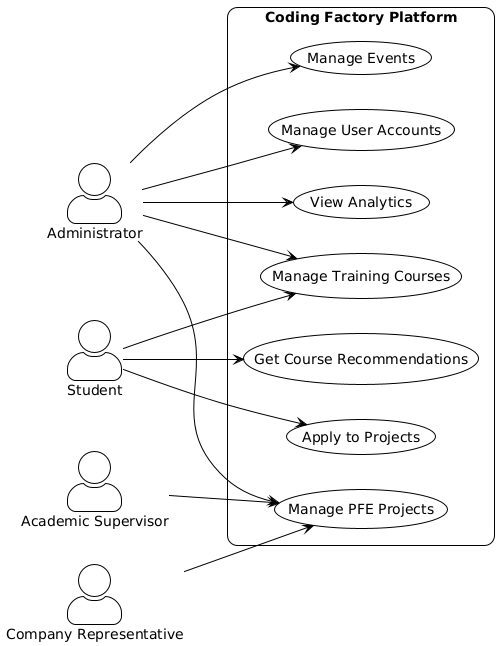
\includegraphics[width=0.9\textwidth]{media/usecase.png}
\caption{Coding Factory Platform Use Case Diagram}
\label{fig:use-case-diagram}
\end{figure}

The Use Case diagram illustrates the key interactions between the system's actors and the platform's functionality:

\begin{itemize}
    \item \textbf{Administrator:} The platform administrator can manage events, user accounts, view analytics, and manage training courses. This role has the highest level of access and control over the system.

    \item \textbf{Student:} Students can manage their training courses, get course recommendations based on sentiment analysis, and apply to projects in the PFE space.

    \item \textbf{Academic Supervisor:} Faculty members who oversee and manage PFE projects, providing academic guidance and evaluation.

    \item \textbf{Company Representative:} External stakeholders who propose and manage PFE projects, offering real-world experience opportunities to students.
\end{itemize}

The diagram shows how these actors interact with the system's core functions, highlighting the role-based access control implemented throughout the platform.

\section{Class Diagram}

\begin{figure}[!htbp]
\centering
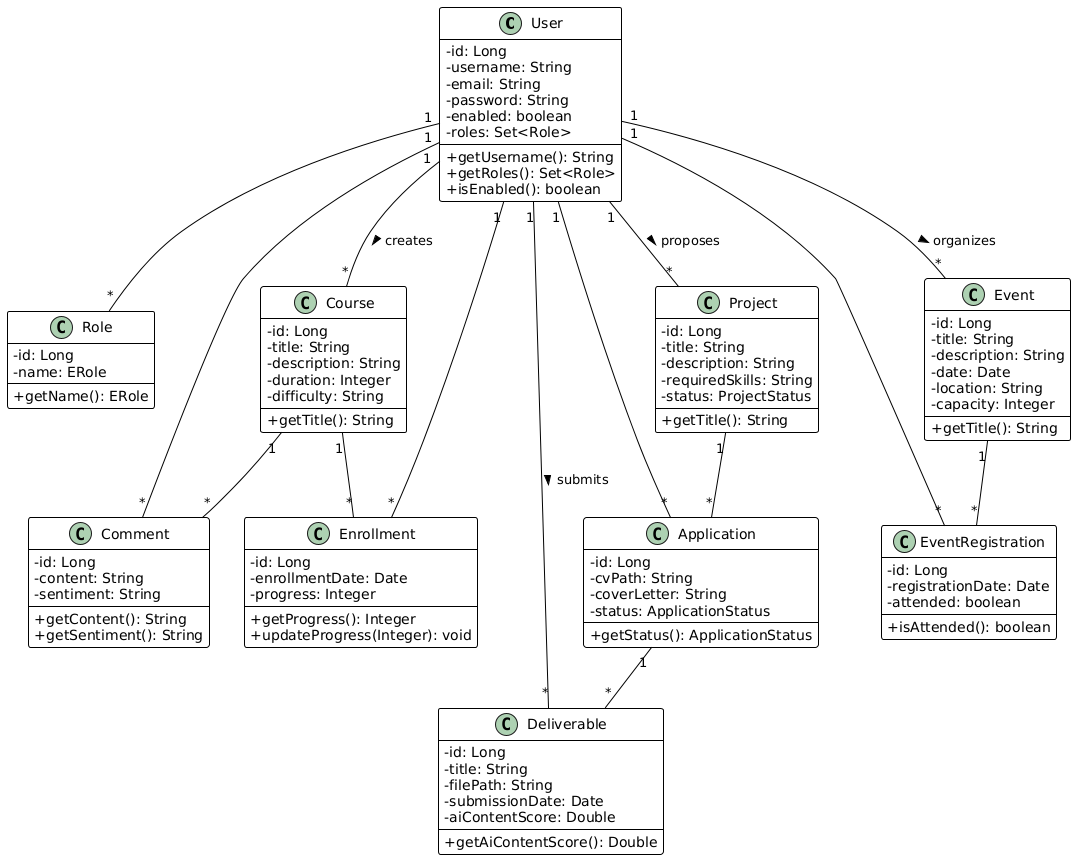
\includegraphics[width=0.9\textwidth]{media/diagramclass.png}
\caption{Coding Factory Platform Class Diagram}
\label{fig:class-diagram}
\end{figure}

The Class Diagram illustrates the key entities in the Coding Factory Platform and their relationships:

\begin{itemize}
    \item \textbf{User:} The central entity representing system users with attributes like id, username, email, password, and enabled status. Users can have multiple roles, create courses, propose projects, organize events, and submit applications.

    \item \textbf{Role:} Defines the different user roles in the system (Admin, Student, Academic Supervisor, Company Representative) with a name attribute of type ERole enumeration.

    \item \textbf{Course:} Represents training courses with attributes including id, title, description, duration, and difficulty level. Courses can have multiple comments and enrollments.

    \item \textbf{Comment:} Stores user feedback on courses with content and sentiment analysis results, enabling the recommendation system to prioritize positively-reviewed courses.

    \item \textbf{Enrollment:} Tracks student enrollment in courses with enrollment date and progress tracking functionality.

    \item \textbf{Project:} Represents end-of-study projects with attributes like id, title, description, required skills, and status. Projects can receive multiple applications.

    \item \textbf{Application:} Manages student applications to projects with CV path, cover letter, and application status tracking.

    \item \textbf{Deliverable:} Represents project submissions with title, file path, submission date, and AI content score for plagiarism detection.

    \item \textbf{Event:} Represents platform events with attributes including id, title, description, date, location, and capacity. Events can have multiple registrations.

    \item \textbf{EventRegistration:} Tracks user registration for events with registration date and attendance status.
\end{itemize}

The diagram shows the relationships between these entities, including one-to-many and many-to-many associations, forming the foundation of the platform's data model.



\chapter{Technical Architecture}

The Coding Factory Platform is built on a modern, scalable architecture that leverages microservices, cloud-native principles, and AI integration. This chapter details the technical implementation of the platform, highlighting the technologies, patterns, and design decisions that enable its functionality.

\section{Technology Stack Overview}

The platform employs a diverse technology stack carefully selected to meet the requirements of a modern educational platform:

\begin{figure}[!htbp]
\centering
\begin{minipage}{0.45\textwidth}
    \centering
    
\includegraphics[width=\textwidth]{media/Angular_full_color_logo.svg.png}
\end{minipage}
\hfill
\begin{minipage}{0.45\textwidth}
    \centering
    
\includegraphics[width=\textwidth]{media/spring-boot-logo.png}
\end{minipage}

\vspace{0.5cm}
\begin{minipage}{0.45\textwidth}
    \centering
    
\includegraphics[width=\textwidth]{media/Python-logo-notext.svg.png}
\end{minipage}
\caption{Key Technologies in the Coding Factory Platform Stack}
\label{fig:tech-stack-diagram}
\end{figure}

\subsection{Core Technologies}

\begin{itemize}
    \item \textbf{Backend:} Java 17, Spring Boot 3.x, Spring Cloud, Spring Security, Spring Data JPA
    \item \textbf{Frontend:} Angular 16, TypeScript, Bootstrap, PrimeNG, RxJS
    \item \textbf{Databases:} PostgreSQL/MySQL for relational data
    \item \textbf{AI Services:} Python 3.8+, Flask, NLTK, Hugging Face API, SBERT
    \item \textbf{DevOps:} Docker for containerization
    \item \textbf{Authentication:} JWT (JSON Web Tokens)
\end{itemize}

This technology stack provides a robust foundation for building a scalable, maintainable, and feature-rich platform while enabling rapid development and deployment.

\section{Frontend Architecture}

The frontend of the Coding Factory Platform is built with Angular 16, providing a responsive and interactive user interface:

\subsection{Key Components}

\begin{itemize}
    \item \textbf{Angular Framework:} Provides component-based architecture, dependency injection, and reactive programming model
    \item \textbf{TypeScript:} Ensures type safety and better code organization
    \item \textbf{Responsive Design:} Bootstrap and custom CSS for mobile-friendly interfaces
    \item \textbf{UI Component Libraries:} PrimeNG and Angular Material for advanced UI components
    \item \textbf{State Management:} RxJS for reactive state management and asynchronous operations
    \item \textbf{Authentication:} @auth0/angular-jwt for token management and secure routes
\end{itemize}

\subsection{Module Organization}

The Angular application is organized into feature modules that align with the platform's main functional areas:

\begin{itemize}
    \item \textbf{Core Module:} Contains singleton services, authentication logic, and guards
    \item \textbf{Shared Module:} Reusable components, directives, and pipes
    \item \textbf{Feature Modules:}
    \begin{itemize}
        \item User Management
        \item Training Management
        \item Event Management
        \item PFE Space
    \end{itemize}
    \item \textbf{Lazy Loading:} Feature modules are lazy-loaded for improved performance
\end{itemize}

This modular approach ensures separation of concerns, improves maintainability, and enables efficient team collaboration.

\section{Backend Architecture}

The backend follows a microservices architecture built with Spring Boot, allowing for independent development, deployment, and scaling of services:

\subsection{Core Microservices}

\begin{itemize}
    \item \textbf{User Management Service (Port 8081):} Handles authentication, authorization, and user profile management using Spring Security and JWT

    \item \textbf{Training Management Service:} Manages courses, educational resources, enrollments, and the recommendation system

    \item \textbf{Event Management Service:} Handles event creation, registration, and attendance tracking

    \item \textbf{PFE Space Service (Port 8080):} Manages projects, applications, deliverables, and AI-powered features for end-of-study projects
\end{itemize}

\subsection{Common Patterns}

Each microservice follows similar patterns and principles:

\begin{itemize}
    \item \textbf{Layered Architecture:} Controller, Service, Repository pattern
    \item \textbf{RESTful APIs:} HTTP-based APIs with REST principles
    \item \textbf{DTO Pattern:} Data Transfer Objects for API communication
    \item \textbf{Exception Handling:} Global handlers for consistent responses
    \item \textbf{Validation:} Input validation with Bean Validation
    \item \textbf{Logging:} Structured logging for monitoring
\end{itemize}

\section{Database Design}

The platform uses relational databases (PostgreSQL/MySQL) with a database-per-service pattern:

\subsection{Key Database Schemas}

\begin{itemize}
    \item \textbf{User Database:} User profiles, roles, and authentication data

    \item \textbf{Training Database:} Courses, resources, enrollments, and comments

    \item \textbf{Event Database:} Events, registrations, and attendance records

    \item \textbf{PFE Database:} Projects, applications, deliverables, and evaluations
\end{itemize}

\subsection{Data Access Approach}

\begin{itemize}
    \item \textbf{ORM:} Spring Data JPA with Hibernate for object-relational mapping
    \item \textbf{Repository Pattern:} Spring Data repositories for data access abstraction
    \item \textbf{Transaction Management:} Declarative transaction management with Spring
    \item \textbf{Auditing:} Entity creation and modification tracking
\end{itemize}

\section{AI Components}

The platform integrates several AI components that enhance its functionality and user experience:

\subsection{Sentiment Analysis for Recommendations}

The sentiment analysis system analyzes training course comments to determine sentiment and rank courses accordingly:

\begin{itemize}
    \item \textbf{Purpose:} Automatically classify course comments as positive, neutral, or negative to improve recommendation quality

    \item \textbf{Technology:} Natural Language Processing with VADER sentiment analyzer and machine learning classification

    \item \textbf{Benefits:}
    \begin{itemize}
        \item Prioritizes highly-rated courses in recommendations
        \item Provides visual sentiment indicators for users
        \item Enables filtering of comments by sentiment
        \item Helps administrators identify trends in course satisfaction
    \end{itemize}
\end{itemize}

\subsection{CV Analysis and Project Matching}

The PFE Space includes an intelligent CV analysis and project matching system:

\begin{itemize}
    \item \textbf{Purpose:} Match students with suitable end-of-study projects based on their skills and experience

    \item \textbf{Technology:} Semantic text matching using SBERT (Sentence-BERT) embeddings

    \item \textbf{Evaluation Criteria:} Multi-dimensional scoring based on education, experience, skills, project relevance, and field match

    \item \textbf{Benefits:}
    \begin{itemize}
        \item Saves time for students searching for relevant projects
        \item Improves match quality between student skills and project requirements
        \item Provides objective evaluation of application fit
        \item Offers personalized improvement suggestions
    \end{itemize}
\end{itemize}

\subsection{AI Content Detection}

The platform includes a plagiarism detection system for ensuring the originality of student submissions:

\begin{itemize}
    \item \textbf{Purpose:} Identify potentially AI-generated content in student deliverables

    \item \textbf{Technology:} Hybrid approach combining local pattern detection and Hugging Face API integration

    \item \textbf{Benefits:}
    \begin{itemize}
        \item Promotes academic integrity
        \item Encourages original work from students
        \item Provides objective assessment of content originality
        \item Includes fallback mechanisms for reliable operation
    \end{itemize}
\end{itemize}

\section{Microservices Architecture}

The platform employs a comprehensive microservices architecture with supporting infrastructure:

\subsection{Service Discovery}

\begin{itemize}
    \item \textbf{Eureka Server:} Centralized service registry for dynamic service discovery
    \item \textbf{Implementation:} Spring Cloud Netflix Eureka
    \item \textbf{Configuration:} Each microservice registers with Eureka on startup
    \item \textbf{Benefits:} Enables location transparency and dynamic scaling
\end{itemize}

\subsection{API Gateway}

\begin{itemize}
    \item \textbf{Gateway Service:} Centralized entry point for all client requests
    \item \textbf{Implementation:} Spring Cloud Gateway
    \item \textbf{Features:}
    \begin{itemize}
        \item Request routing to appropriate microservices
        \item Load balancing across service instances
        \item Cross-cutting concerns (logging, security)
    \end{itemize}
    \item \textbf{Configuration:} Route definitions in application.properties
\end{itemize}

\subsection{Service Communication}

\begin{itemize}
    \item \textbf{Synchronous Communication:} REST APIs with RestTemplate/WebClient
    \item \textbf{Cross-Service Authentication:} JWT token forwarding
    \item \textbf{Service URLs:} Configured via properties with fallback defaults
    \item \textbf{Error Handling:} Circuit breakers for fault tolerance
\end{itemize}

\section{Data Flow \& Integration}

The platform integrates multiple components and services to provide a seamless user experience:

\subsection{System Integration Points}

\begin{itemize}
    \item \textbf{Frontend-Backend Integration:} Angular services communicate with backend APIs

    \item \textbf{Microservice Integration:}
    \begin{itemize}
        \item PFE Space integrates with User Service for authentication
        \item Training Service integrates with Python Sentiment Analysis API
    \end{itemize}

    \item \textbf{External AI Integration:}
    \begin{itemize}
        \item Hugging Face API for AI content detection
        \item SBERT for semantic matching
    \end{itemize}
\end{itemize}

\subsection{Data Exchange Formats}

\begin{itemize}
    \item \textbf{API Communication:} JSON for all API requests and responses
    \item \textbf{File Uploads:} Multipart form data for CV and document uploads
    \item \textbf{Internal Data:} Java objects mapped to/from JSON using Jackson
\end{itemize}

\subsection{Security Considerations}

\begin{itemize}
    \item \textbf{Authentication:} JWT-based authentication with secure token handling
    \item \textbf{Authorization:} Role-based access control (RBAC) for different user types
    \item \textbf{API Security:} CORS configuration, CSRF protection
    \item \textbf{Data Protection:} Secure password storage with encryption
\end{itemize}

The technical architecture of the Coding Factory Platform demonstrates a modern approach to building scalable, maintainable educational technology solutions. By leveraging microservices, AI integration, and cloud-native principles, the platform provides a solid foundation for current functionality while enabling future growth.

\chapter{System Demonstration}

This chapter provides a visual tour of the Coding Factory Platform, highlighting key interfaces, user journeys, and AI-powered features. Through screenshots and workflow descriptions, we demonstrate how the platform delivers value to different user types.

\section{User Interface \& Screenshots}

The Coding Factory Platform features a modern, responsive interface designed for intuitive navigation and efficient task completion. This section showcases key interfaces from the platform.

\subsection{Landing Page}

\begin{figure}[!htbp]
\centering

\includegraphics[width=0.9\textwidth]{media/Landing Page.png}
\caption{Coding Factory Platform Landing Page}
\label{fig:landing-page}
\end{figure}

The landing page serves as the primary entry point to the platform, featuring:

\begin{itemize}
    \item Clean, modern design with the Coding Factory branding
    \item Prominent call-to-action buttons for registration and login

\end{itemize}

\subsection{User Authentication}

\begin{figure}[!htbp]
\centering
\begin{minipage}{0.45\textwidth}
    \centering
    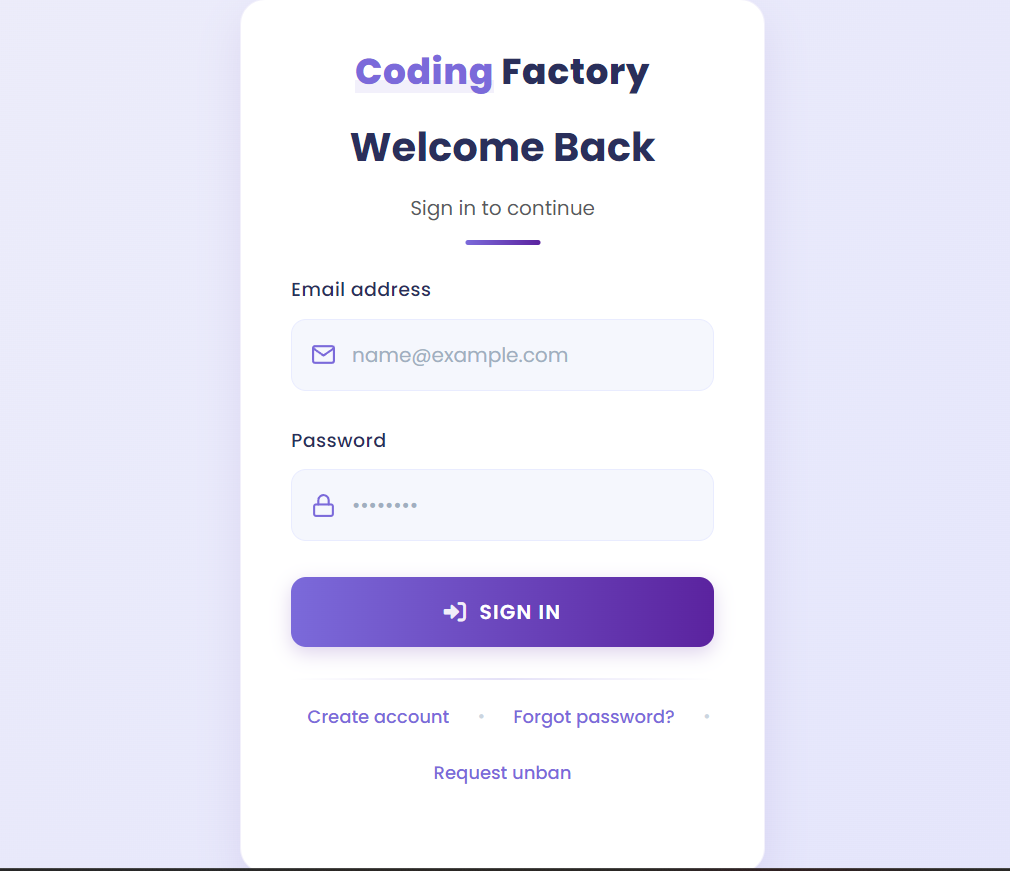
\includegraphics[width=\textwidth]{media/signin.png}
\end{minipage}
\hfill
\begin{minipage}{0.45\textwidth}
    \centering
    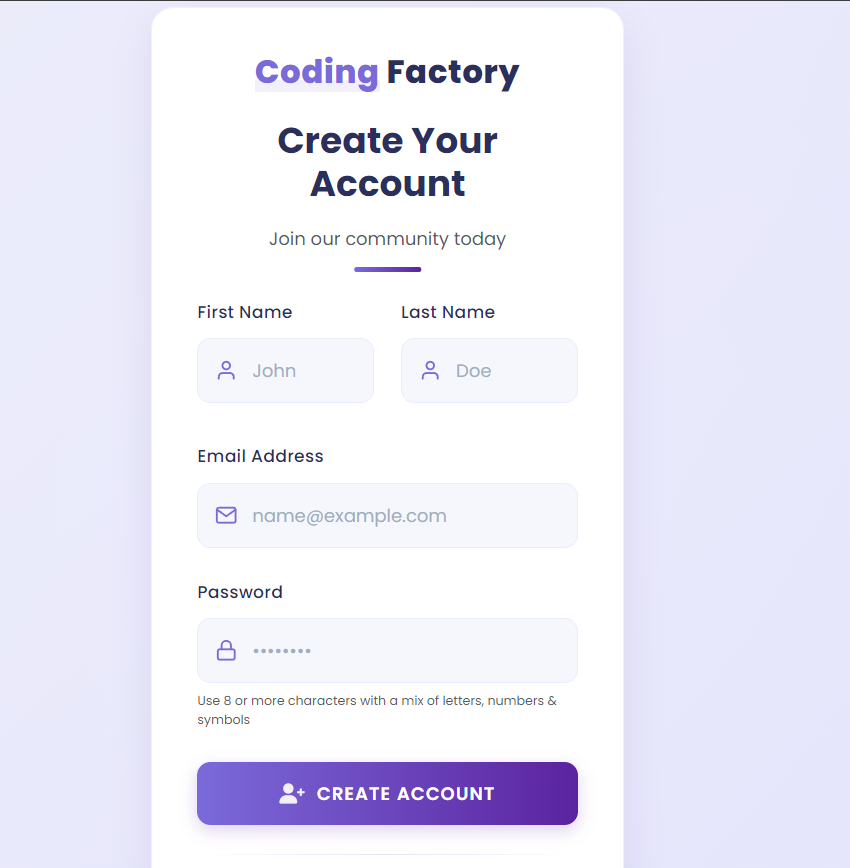
\includegraphics[width=\textwidth]{media/create account.png}
\end{minipage}

\vspace{0.5cm}
\begin{minipage}{0.45\textwidth}
    \centering
    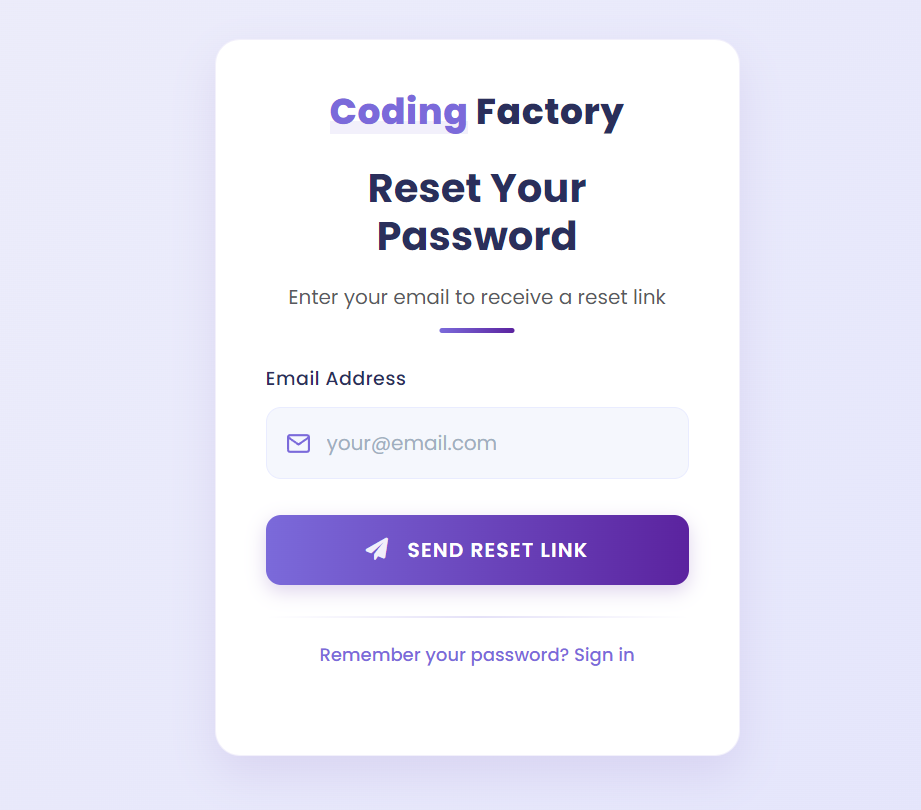
\includegraphics[width=\textwidth]{media/reset password.png}
\end{minipage}
\caption{User Authentication Interfaces: Sign In, Registration, and Password Reset}
\label{fig:auth-interfaces}
\end{figure}

The authentication interfaces provide:

\begin{itemize}
    \item Secure login with email/password
    \item New user registration with email verification
    \item Password recovery functionality
    \item Account activation process
    \item Consistent design matching the platform's visual identity
\end{itemize}

\subsection{Training Management Interface}

\begin{figure}[!htbp]
\centering
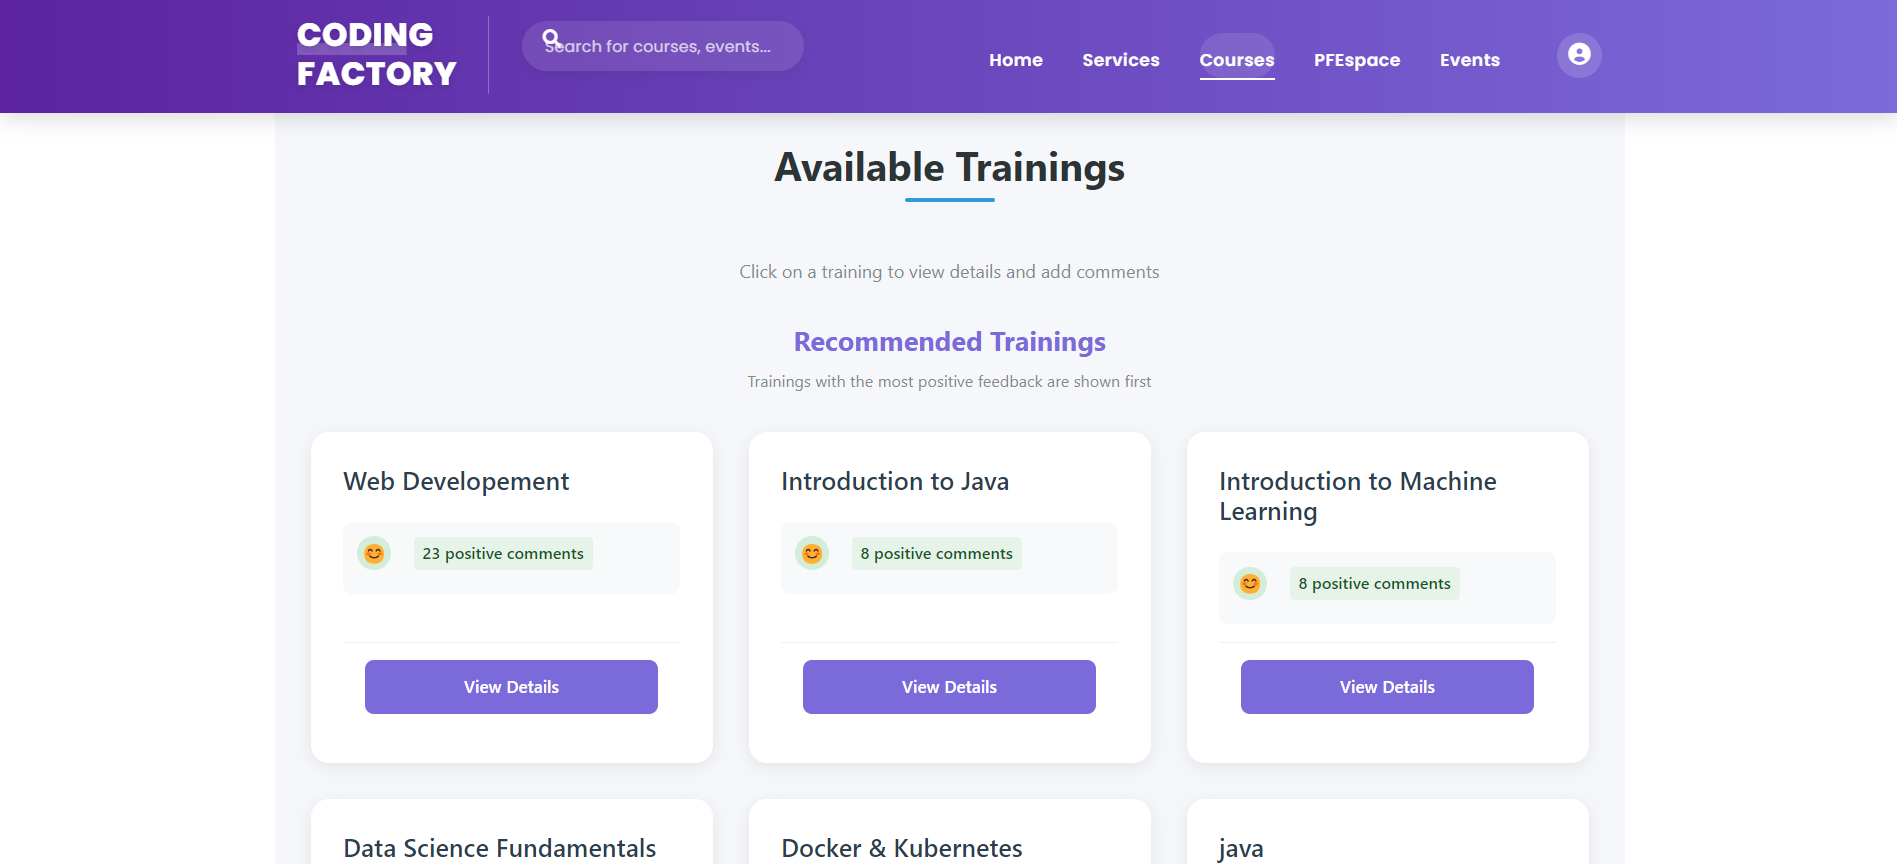
\includegraphics[width=0.9\textwidth]{media/courses.png}
\caption{Training Management Dashboard: Course Catalog}
\label{fig:training-dashboard}
\end{figure}

The training management interface provides:

\begin{itemize}
    \item Personalized course recommendations based on sentiment analysis
    \item Comprehensive course catalog with filtering options
    \item Detailed course information including descriptions, prerequisites, and ratings
    \item Enrollment management and progress tracking
    \item Comment and feedback submission functionality
\end{itemize}

\begin{figure}[!htbp]
\centering
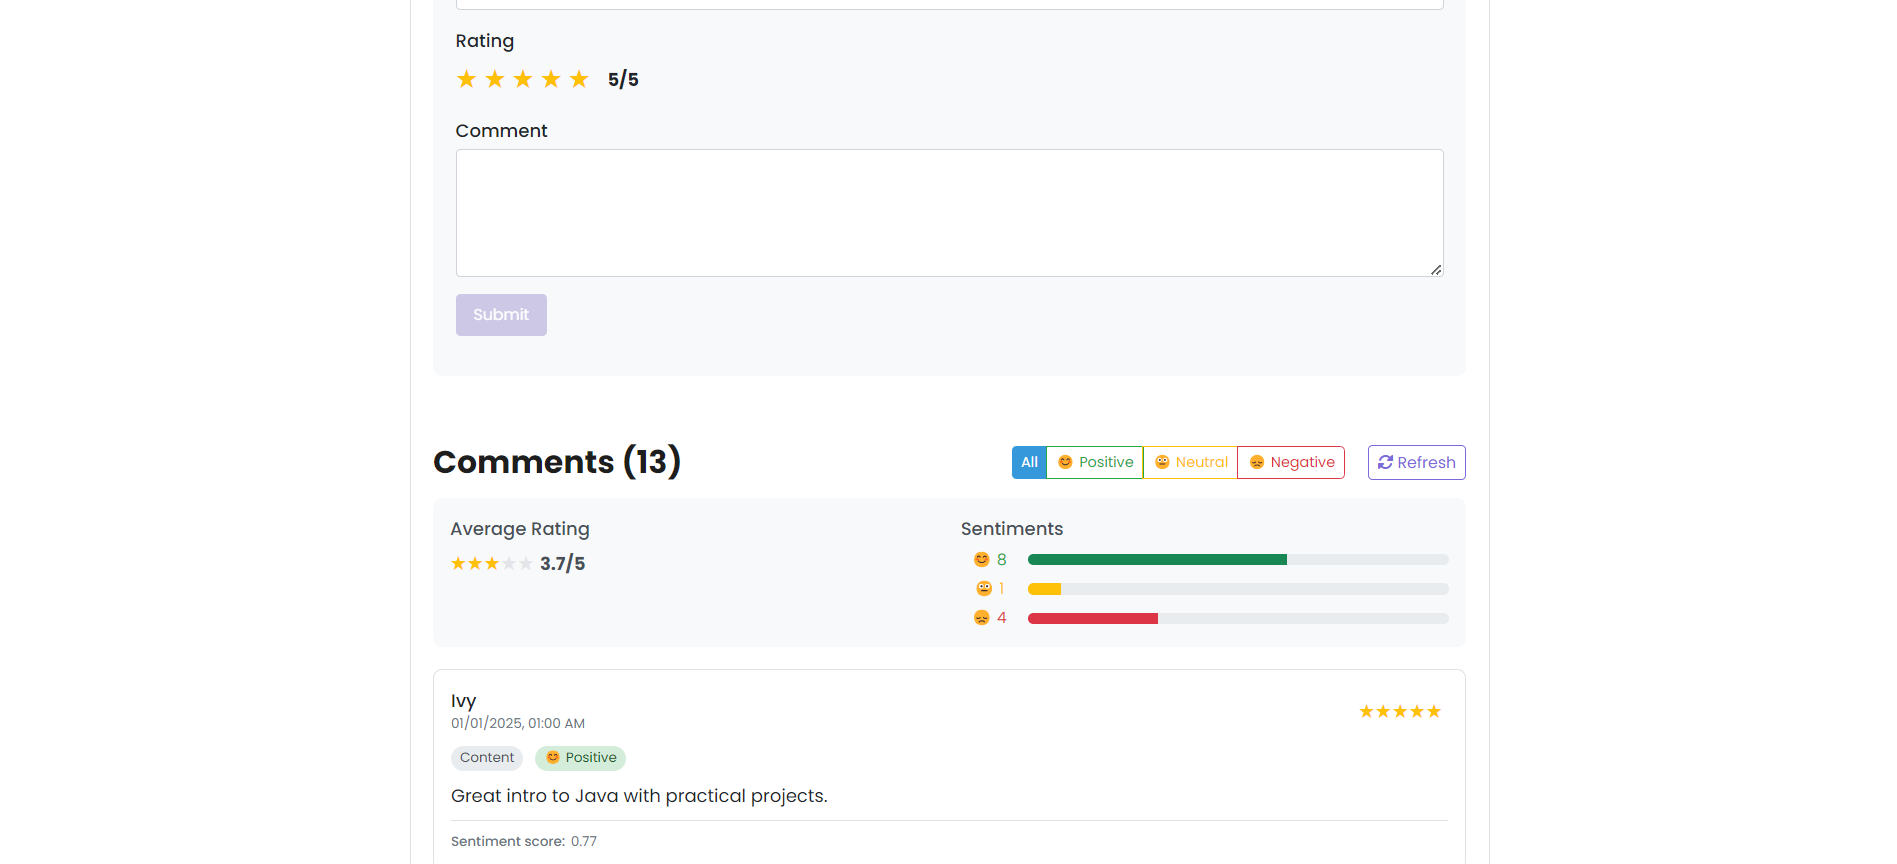
\includegraphics[width=0.9\textwidth]{media/sentiment analysis.png}
\caption{Sentiment Analysis for Course Comments}
\label{fig:sentiment-analysis}
\end{figure}

\subsection{PFE Space Interface}

\begin{figure}[!htbp]
\centering
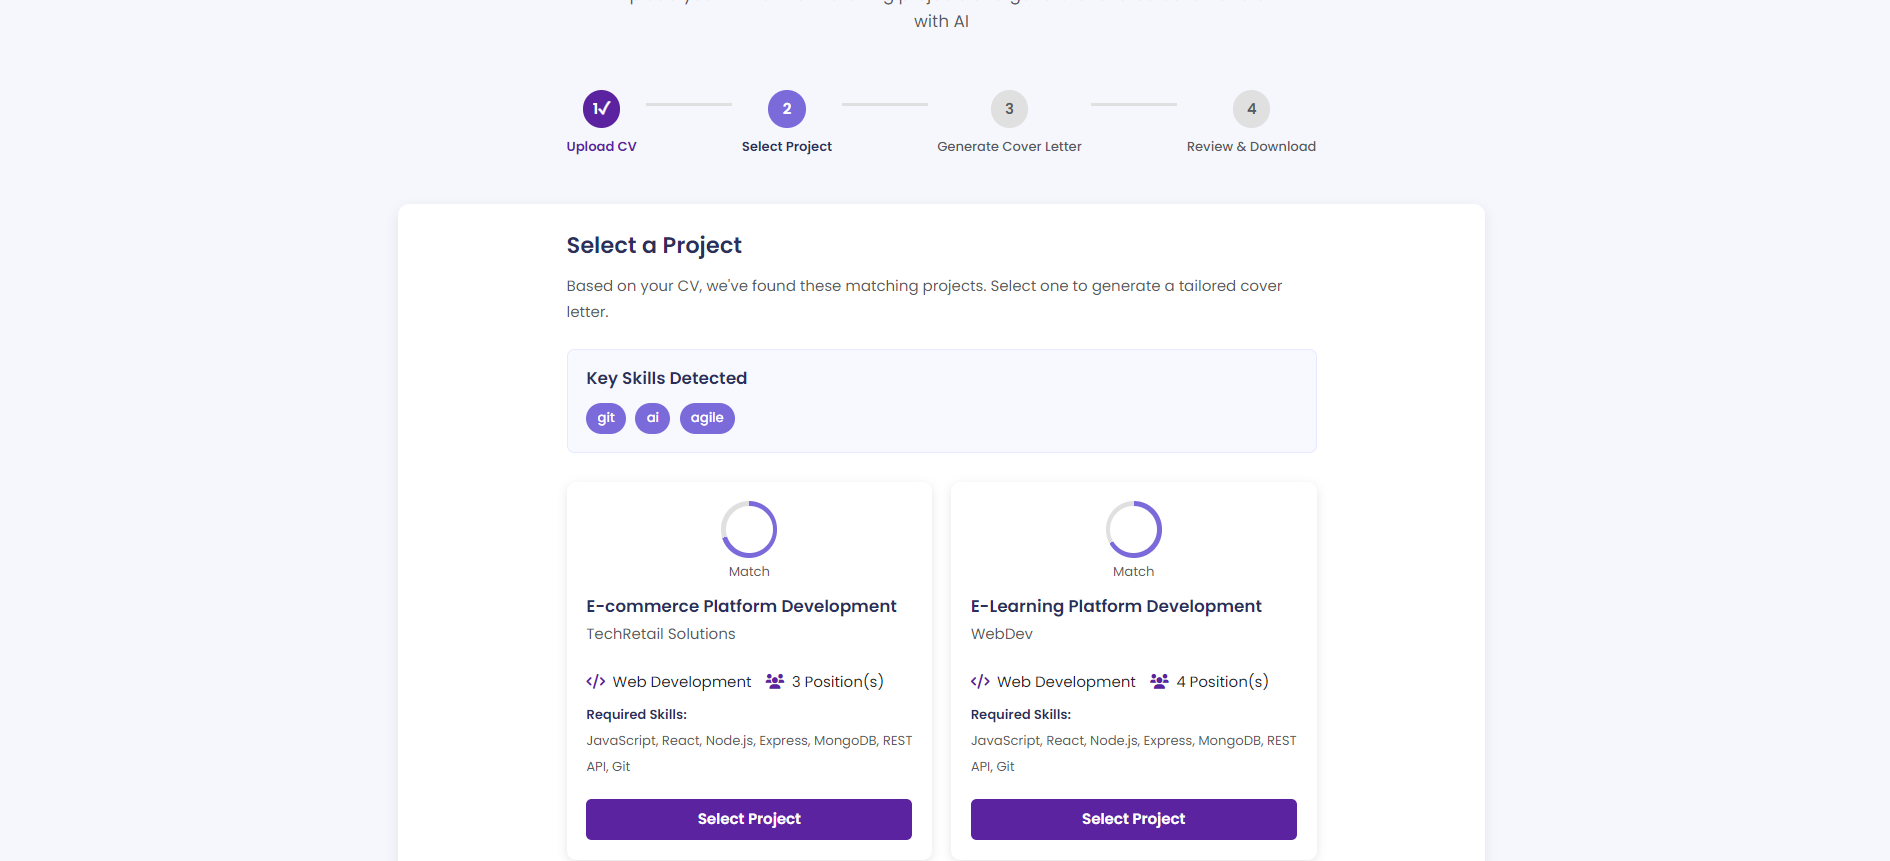
\includegraphics[width=0.9\textwidth]{media/project match.png}
\caption{PFE Space Project Matching Interface}
\label{fig:pfe-interface}
\end{figure}

The PFE Space interface features:

\begin{itemize}
    \item Project browsing and filtering capabilities
    \item CV upload and analysis visualization
    \item Project matching results with relevance scores
    \item Application submission and tracking
    \item Deliverable management and evaluation
\end{itemize}

\begin{figure}[!htbp]
\centering
\begin{minipage}{0.45\textwidth}
    \centering
    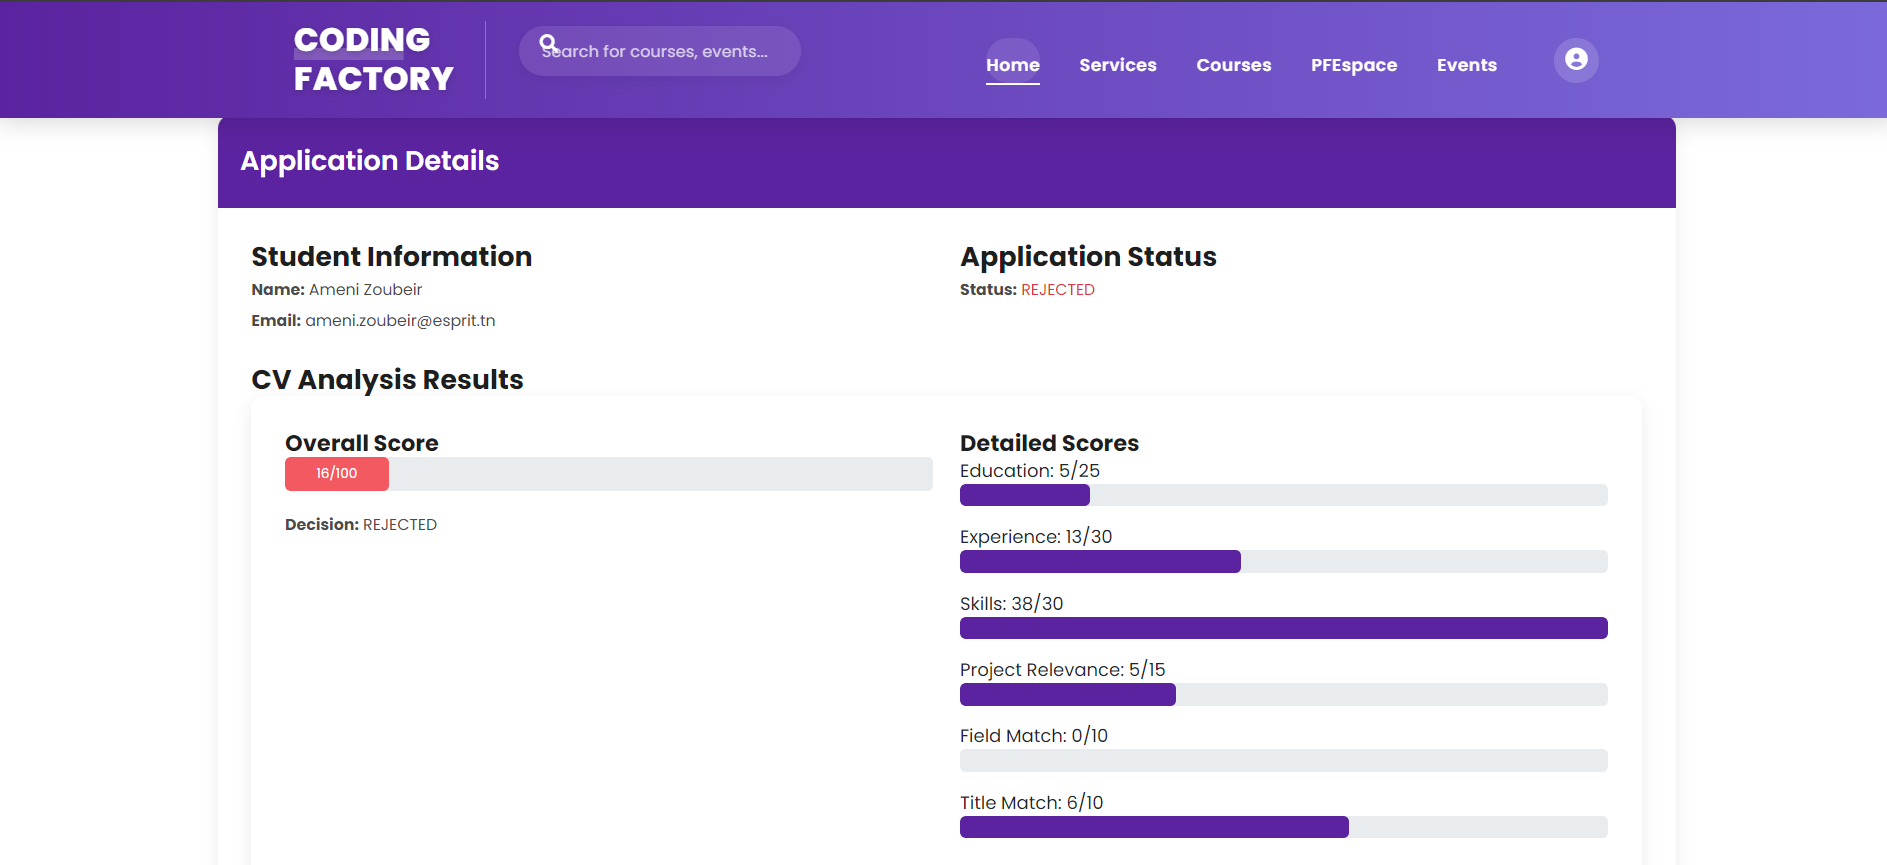
\includegraphics[width=\textwidth]{media/cv analysis.png}
    \caption{CV Analysis Results}
    \label{fig:cv-analysis}
\end{minipage}
\hfill
\begin{minipage}{0.45\textwidth}
    \centering
    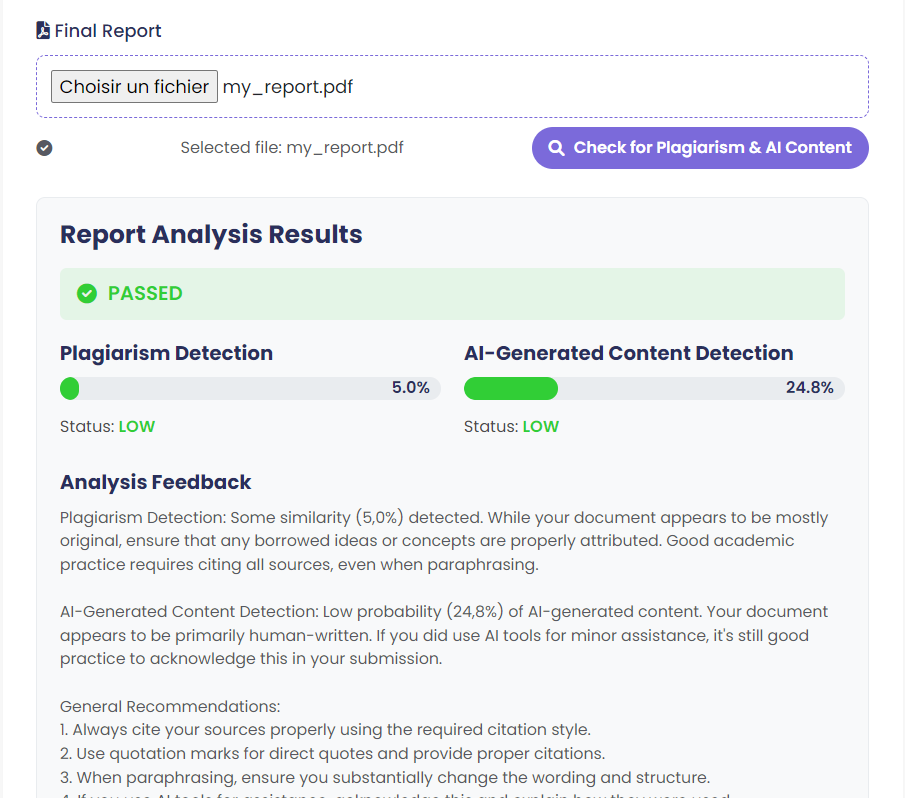
\includegraphics[width=\textwidth]{media/plagiat.png}
    \caption{AI Content Detection}
    \label{fig:plagiarism}
\end{minipage}
\end{figure}

\subsection{Event Management}

\begin{figure}[!htbp]
\centering
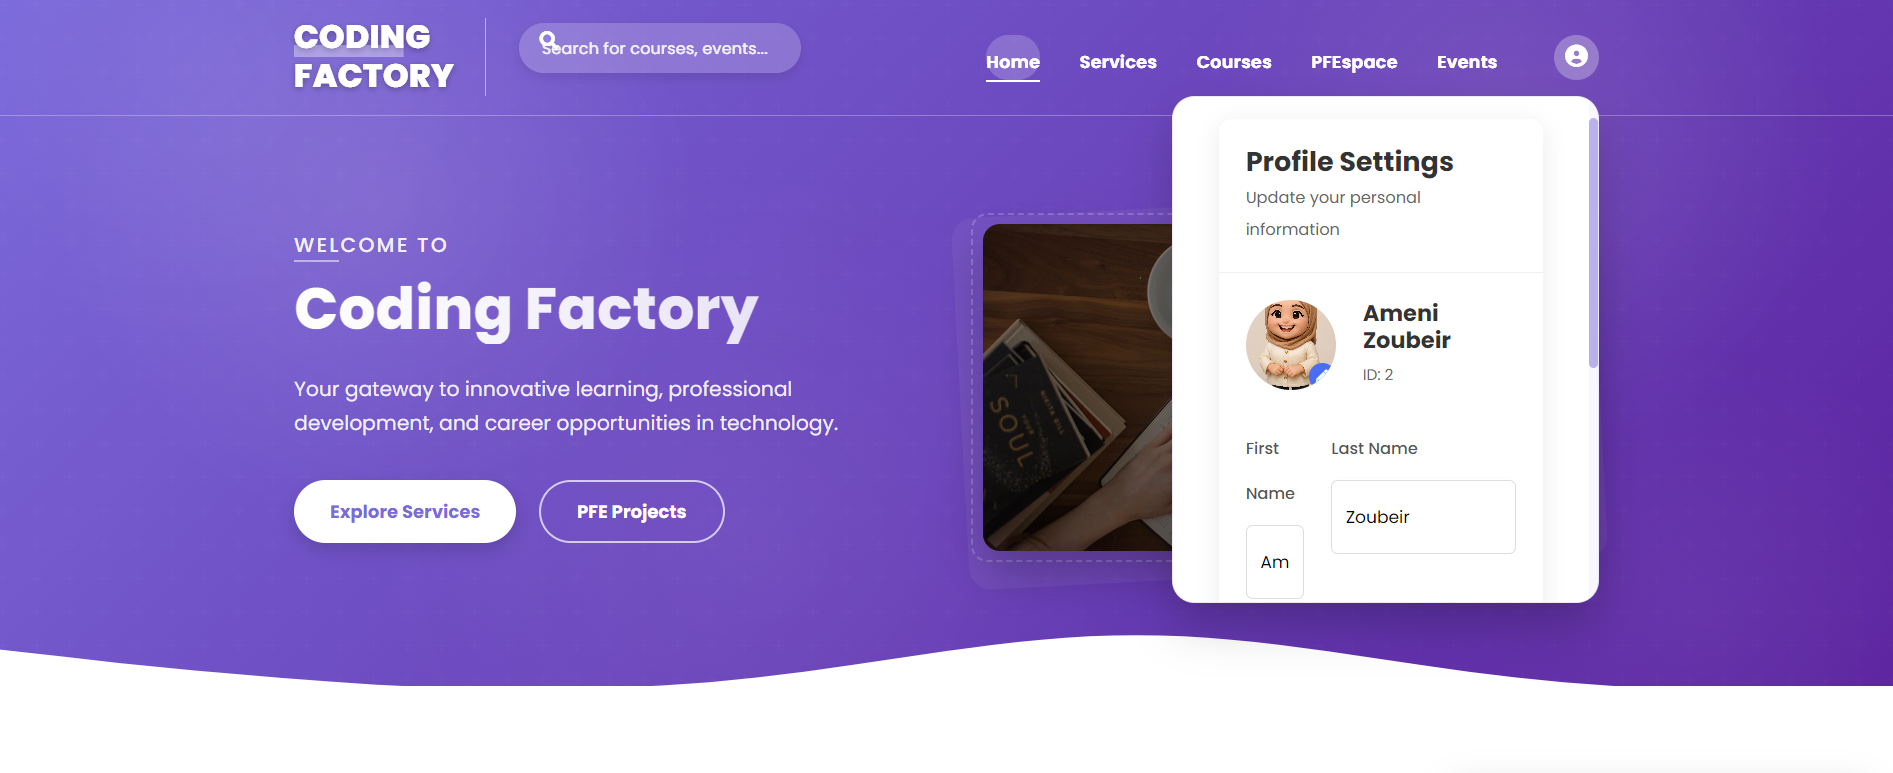
\includegraphics[width=0.9\textwidth]{media/profile.png}
\caption{User Profile and Event Management Interface}
\label{fig:event-interface}
\end{figure}

The event management interface includes:

\begin{itemize}
    \item Event calendar with upcoming workshops, webinars, and meetups
    \item Event details with descriptions, schedules, and locations
    \item Registration functionality with confirmation
    \item Attendance tracking for participants
    \item Post-event feedback collection
\end{itemize}

\subsection{Admin Dashboard}

\begin{figure}[!htbp]
\centering
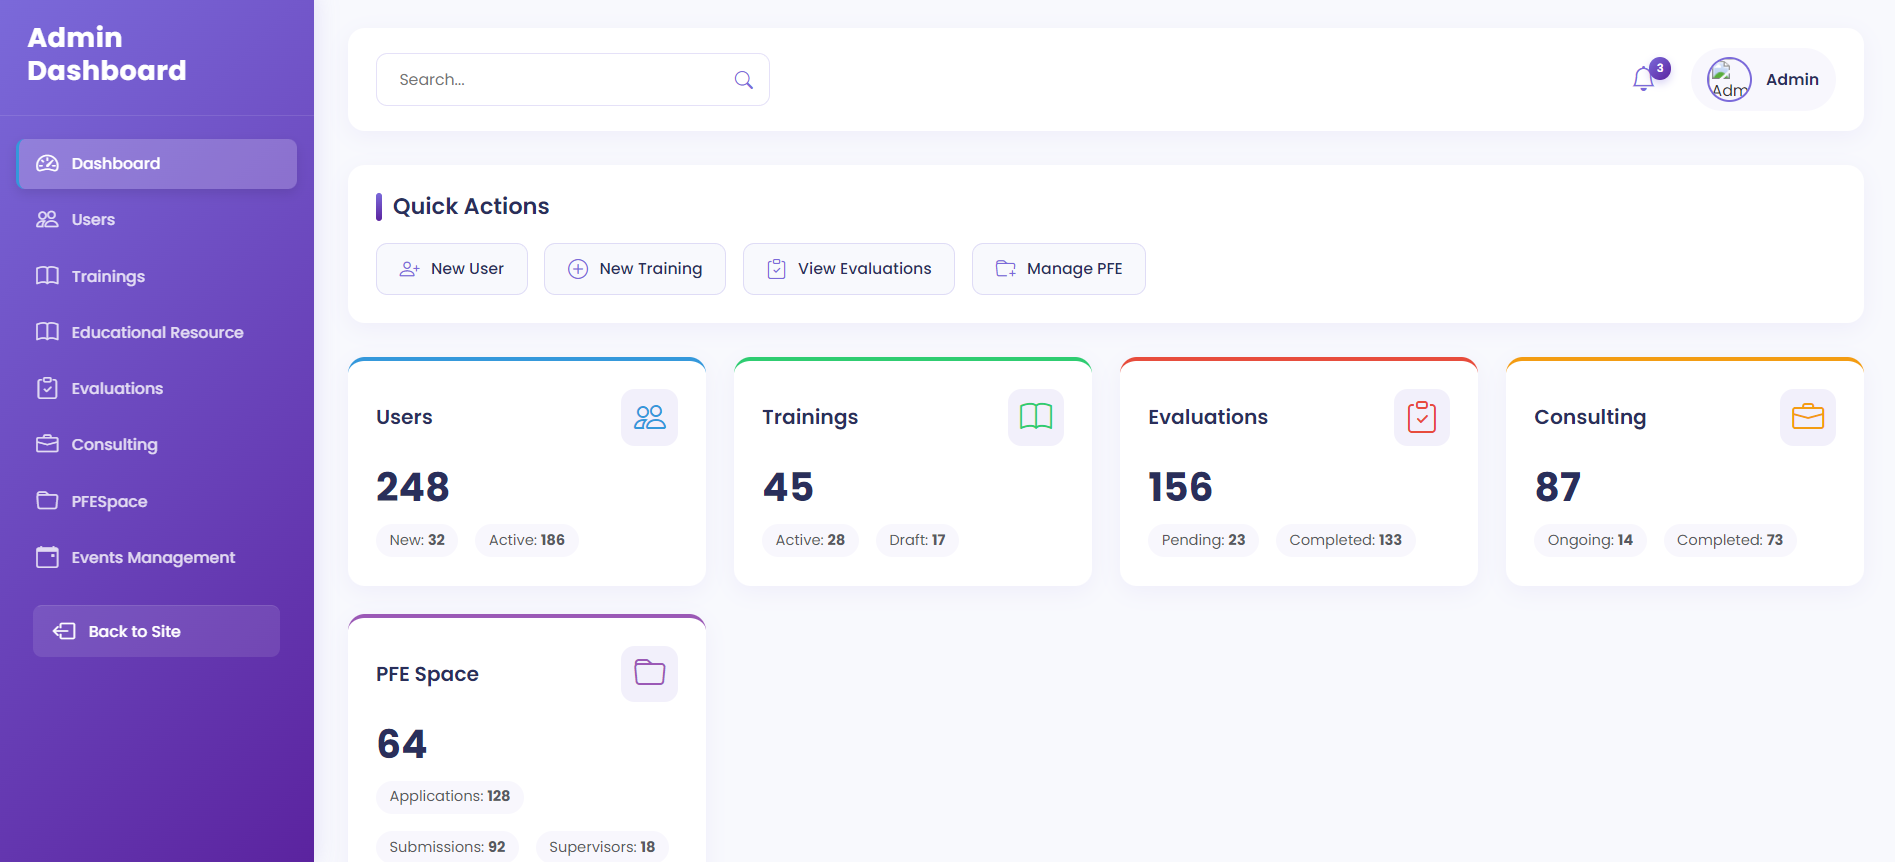
\includegraphics[width=0.9\textwidth]{media/admin dashboard.png}
\caption{Administrator Dashboard}
\label{fig:admin-dashboard}
\end{figure}

The administrator dashboard provides:

\begin{itemize}
    \item Platform usage analytics and metrics
    \item User management tools
    \item Content management for courses and resources
    \item System configuration options
    \item Comprehensive reporting capabilities
\end{itemize}

\section{Key User Journeys}

This section illustrates the typical workflows for different user types, demonstrating how the platform supports their specific needs and objectives.

\subsection{Student Journey}

A typical student journey through the platform includes:

\begin{enumerate}
    \item \textbf{Registration and Profile Creation:} Students register and create profiles with their educational background, skills, and interests.

    \item \textbf{Course Discovery:} Students browse the course catalog and receive personalized recommendations based on their profile and course sentiment analysis.

    \item \textbf{Course Enrollment:} Students enroll in selected courses and access educational resources.

    \item \textbf{Learning and Progress Tracking:} Students complete course materials and track their progress through the platform.

    \item \textbf{Feedback Submission:} Students provide comments and ratings on completed courses, contributing to the sentiment analysis system.

    \item \textbf{PFE Project Exploration:} Students browse available end-of-study projects in the PFE Space.

    \item \textbf{CV Analysis and Project Matching:} Students upload their CVs for analysis and receive project recommendations based on their skills and experience.

    \item \textbf{Project Application:} Students apply to suitable projects with their analyzed CV and generated cover letter.

    \item \textbf{Project Completion:} Students submit deliverables and receive evaluations from supervisors.
\end{enumerate}

\subsection{Admin Journey}

Administrators use the platform to manage all aspects of the educational ecosystem:

\begin{enumerate}
    \item \textbf{User Management:} Admins create, modify, and manage user accounts and permissions.

    \item \textbf{Course Management:} Admins create and update training courses, add educational resources, and monitor enrollments.

    \item \textbf{Event Management:} Admins schedule and organize events, track registrations, and manage attendance.

    \item \textbf{Analytics Dashboard:} Admins access comprehensive analytics on platform usage, course popularity, and sentiment analysis results.

    \item \textbf{PFE Project Oversight:} Admins review and approve project offers from companies and academic supervisors.

    \item \textbf{System Configuration:} Admins configure system settings and manage integrations with external services.
\end{enumerate}

\section{AI Features Demonstration}

The Coding Factory Platform incorporates several AI-powered features that enhance the user experience and provide intelligent functionality.

\subsection{Sentiment Analysis in Action}

The sentiment analysis system analyzes course comments to determine sentiment and influence course recommendations:

\begin{figure}[!htbp]
\centering
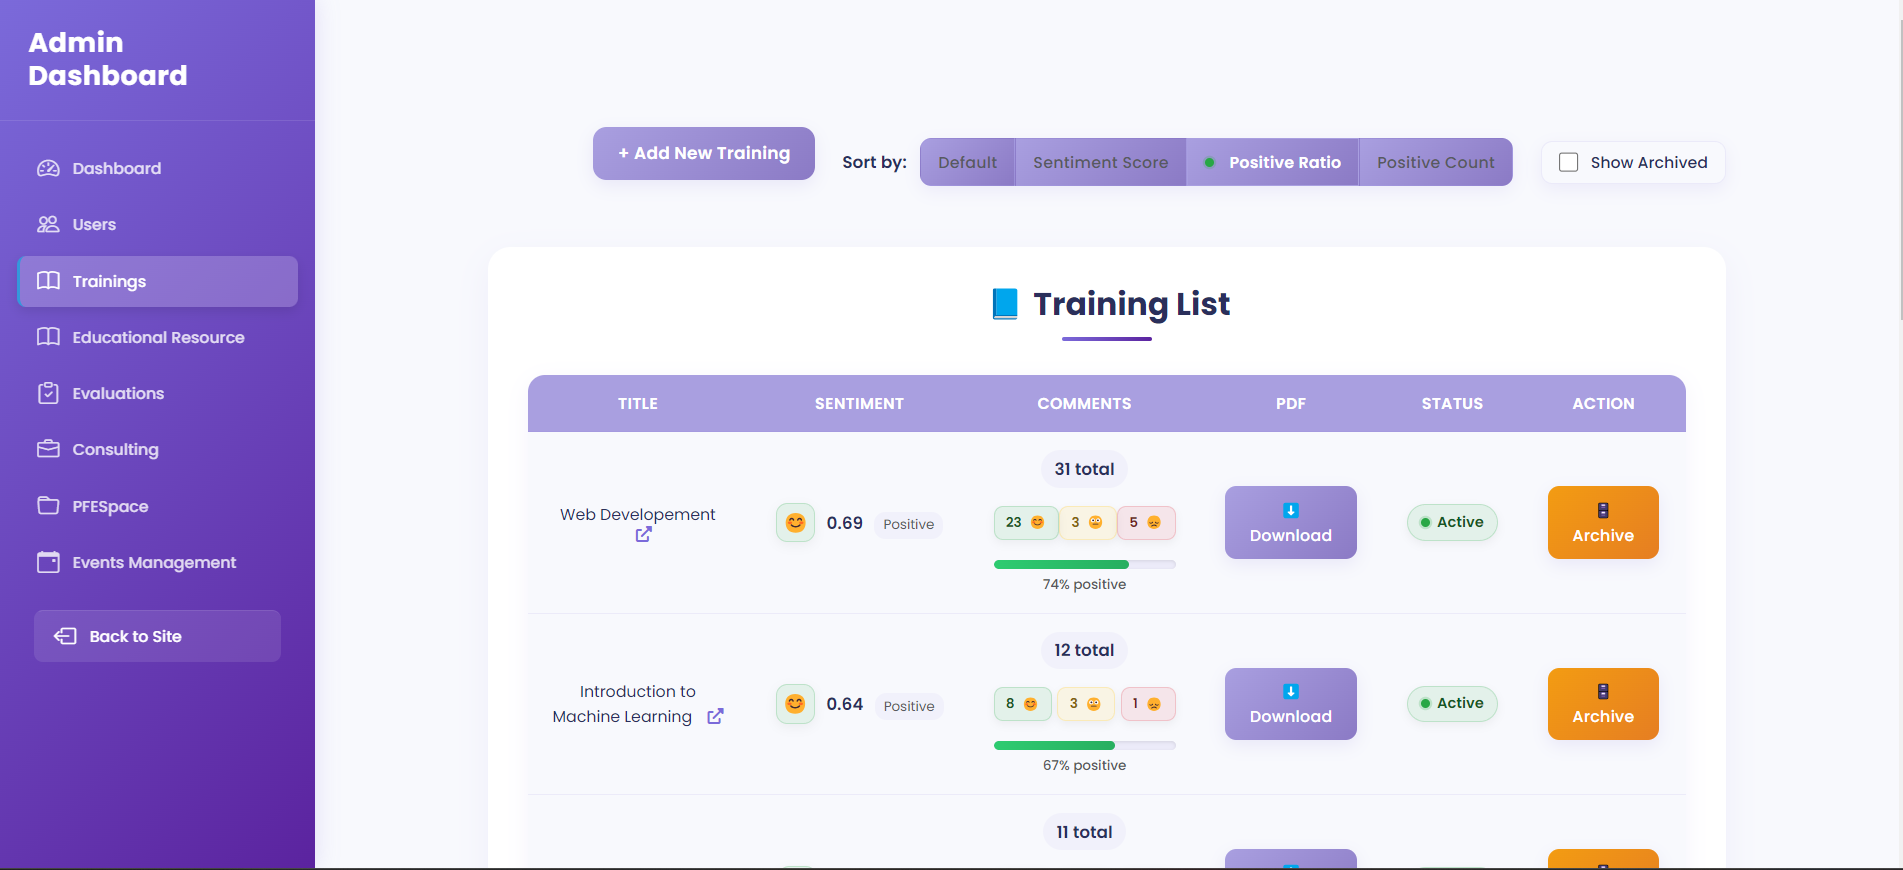
\includegraphics[width=0.9\textwidth]{media/snetiment anlysis.png}
\caption{Sentiment Analysis Visualization for Course Comments}
\label{fig:sentiment-analysis-viz}
\end{figure}

Key aspects of the sentiment analysis feature include:

\begin{itemize}
    \item \textbf{Comment Classification:} Comments are automatically classified as positive, neutral, or negative.

    \item \textbf{Sentiment Indicators:} Visual indicators show the sentiment distribution for each course.

    \item \textbf{Filtering Options:} Users can filter comments by sentiment to focus on specific feedback types.

    \item \textbf{Sentiment Trends:} Administrators can track sentiment trends over time to identify improvements or issues.
\end{itemize}

\subsection{Course Recommendation System}

The recommendation system leverages sentiment analysis to suggest relevant courses to students:

\begin{figure}[!htbp]
\centering
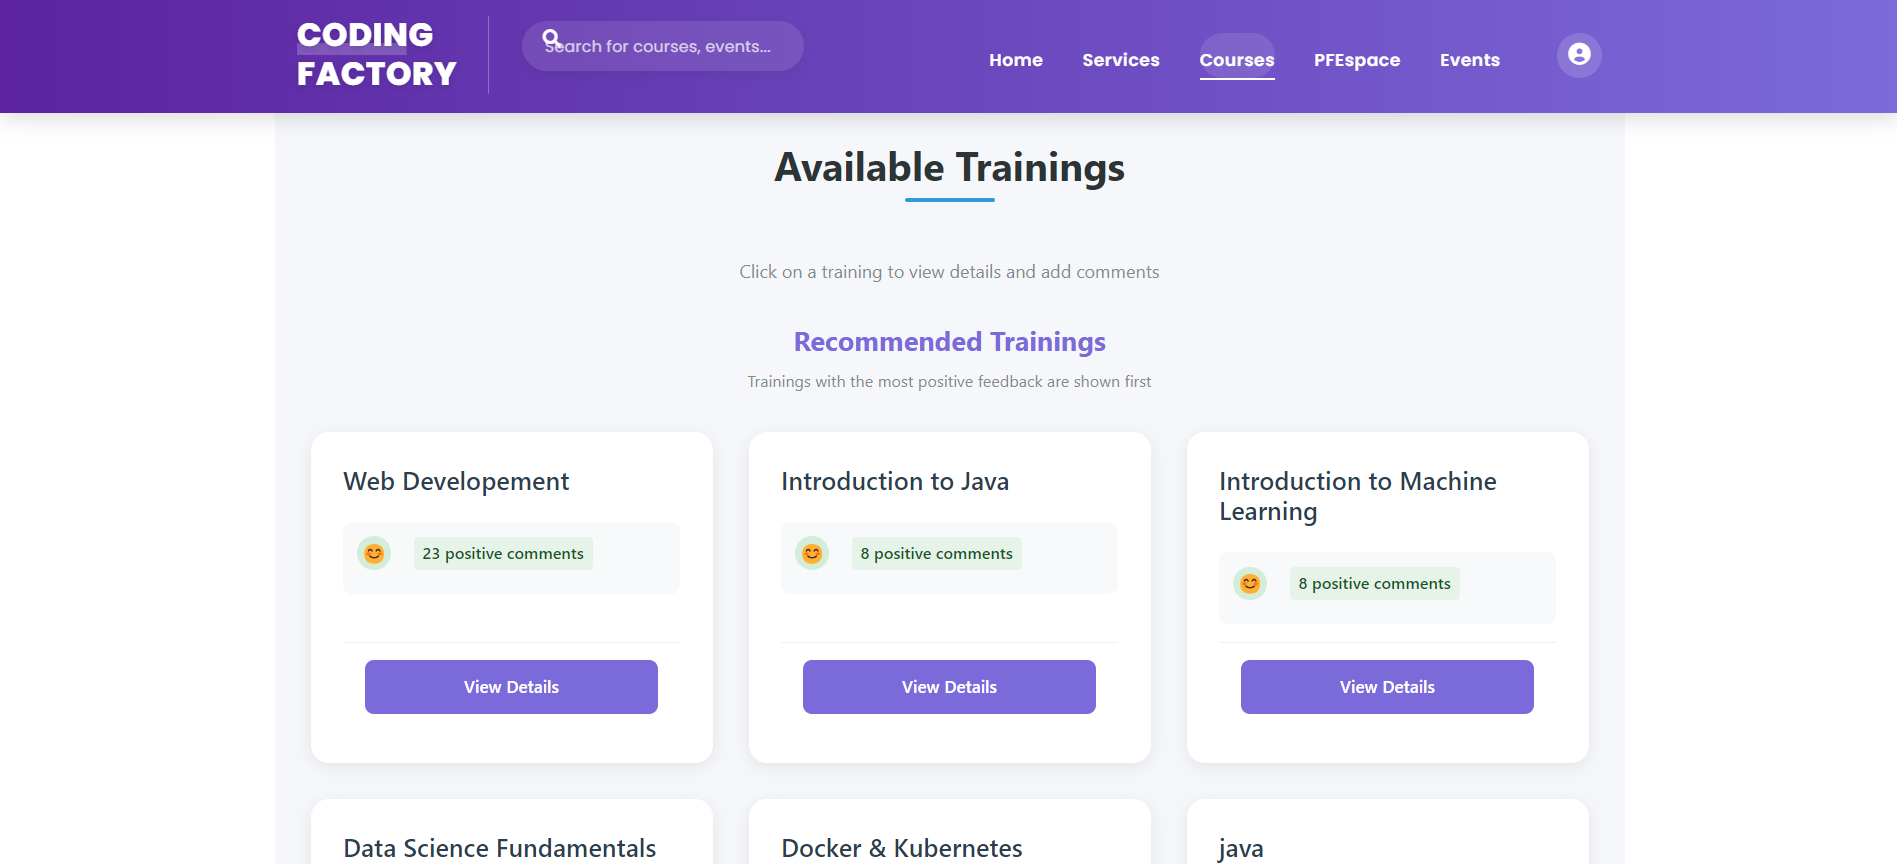
\includegraphics[width=0.9\textwidth]{media/courses.png}
\caption{Personalized Course Recommendations}
\label{fig:course-recommendations}
\end{figure}

The system features:

\begin{itemize}
    \item \textbf{Personalized Suggestions:} Courses are recommended based on user profile and interests.

    \item \textbf{Sentiment-Based Ranking:} Courses with positive sentiment are prioritized in recommendations.

    \item \textbf{Relevance Indicators:} Visual indicators show why specific courses are recommended.

    \item \textbf{Exploration Options:} Users can explore alternative recommendations and adjust preferences.
\end{itemize}

\subsection{PFE Matching Process}

The PFE matching system uses AI to connect students with suitable projects:

\begin{figure}[!htbp]
\centering
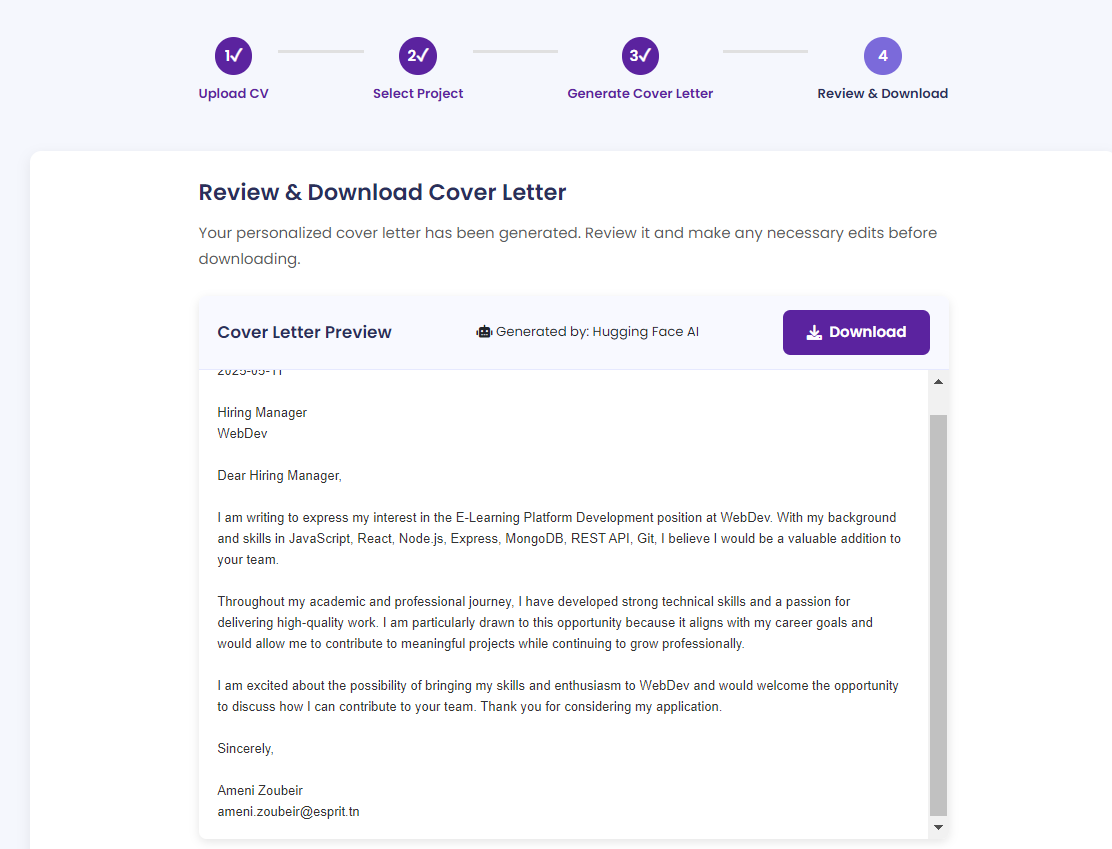
\includegraphics[width=0.9\textwidth]{media/cover letter.png}
\caption{Cover Letter Generation Based on CV Analysis}
\label{fig:cv-matching}
\end{figure}

The PFE matching process demonstrates:

\begin{itemize}
    \item \textbf{CV Analysis Visualization:} Detailed breakdown of CV evaluation across multiple dimensions.

    \item \textbf{Skill Extraction:} Automatic identification of key skills from CV text.

    \item \textbf{Project Matching:} Ranked list of projects with compatibility scores.

    \item \textbf{Improvement Suggestions:} Personalized recommendations for improving CV-project fit.

    \item \textbf{Cover Letter Generation:} AI-assisted creation of tailored cover letters for project applications.
\end{itemize}

Through these demonstrations, we illustrate how the Coding Factory Platform combines intuitive user interfaces with powerful AI capabilities to create a comprehensive educational technology solution that meets the needs of students, administrators, and industry partners.

\chapter{Commercial Impact}

Beyond its technical achievements, the Coding Factory Platform represents a significant commercial opportunity in the educational technology market. This chapter examines the platform's value proposition, market potential, and strategies for sustainable growth.

\section{Value Proposition}

The Coding Factory Platform delivers compelling value to multiple stakeholder groups:

\subsection{For Students}

\begin{itemize}
    \item \textbf{Personalized Learning:} AI-powered course recommendations based on interests and sentiment analysis create tailored educational pathways.

    \item \textbf{Career Advancement:} The PFE Space connects students with real-world projects and potential employers, bridging the gap between education and employment.

    \item \textbf{Skill Development:} Comprehensive training courses and resources help students build in-demand technical skills.

    \item \textbf{Intelligent Guidance:} CV analysis and project matching provide data-driven career guidance and project selection.

    \item \textbf{Community Engagement:} Events and collaborative features foster a sense of belonging and professional networking.
\end{itemize}

\subsection{For Educational Institutions}

\begin{itemize}
    \item \textbf{Enhanced Offering:} The platform extends traditional educational offerings with modern, technology-driven learning experiences.

    \item \textbf{Administrative Efficiency:} Comprehensive management tools streamline course administration, user management, and event organization.

    \item \textbf{Data-Driven Insights:} Analytics and sentiment analysis provide valuable feedback for continuous improvement.

    \item \textbf{Industry Connections:} The PFE Space creates structured partnerships with companies and industry partners.

    \item \textbf{Competitive Differentiation:} AI-powered features distinguish the institution from competitors in the educational market.
\end{itemize}

\subsection{For Companies and Industry Partners}

\begin{itemize}
    \item \textbf{Talent Pipeline:} Access to a pool of pre-screened students with verified skills and project experience.

    \item \textbf{Project Collaboration:} Opportunity to propose real-world projects and engage with students on practical challenges.

    \item \textbf{Recruitment Efficiency:} CV analysis and skill matching reduce the time and cost of identifying suitable candidates.

    \item \textbf{Brand Visibility:} Presence on the platform enhances company visibility among future technology professionals.

    \item \textbf{Educational Contribution:} Ability to influence educational content and help shape the skills of future workforce.
\end{itemize}

\section{Market Analysis}

\subsection{Target Market Segments}

The Coding Factory Platform addresses several key market segments:

\begin{itemize}
    \item \textbf{Higher Education Institutions:} Universities and colleges seeking to enhance their technical education offerings.

    \item \textbf{Professional Training Centers:} Organizations focused on upskilling and reskilling professionals in technology fields.

    \item \textbf{Corporate Learning Departments:} Companies looking to train employees on technical skills and manage internal projects.

    \item \textbf{Individual Learners:} Self-directed students seeking to build technical skills for career advancement.

    \item \textbf{Technology Companies:} Organizations looking to identify and recruit technical talent.
\end{itemize}

\subsection{Market Size and Growth}

The global educational technology market represents a significant opportunity:

\begin{itemize}
    \item The global EdTech market is projected to reach \$404 billion by 2025, growing at a CAGR of 16.3\%.

    \item The coding education segment is expected to reach \$12.4 billion by 2027, with a CAGR of 19.2\%.

    \item Corporate technical training exceeds \$20 billion globally, with increasing demand for specialized skills.

    \item The AI in education market is growing at 45\% annually, reaching \$20.8 billion by 2028.
\end{itemize}

\section{Monetization Opportunities}

The Coding Factory Platform offers multiple revenue streams for sustainable operation and growth:

\subsection{Subscription Models}

\begin{itemize}
    \item \textbf{Tiered Institutional Subscriptions:} Educational institutions can subscribe to different service levels based on their needs and student population.

    \item \textbf{Individual Learning Subscriptions:} Students can access premium features and content through monthly or annual subscriptions.

    \item \textbf{Corporate Partnerships:} Companies can subscribe for privileged access to the talent pool and project submission capabilities.
\end{itemize}

\subsection{Transaction-Based Revenue}

\begin{itemize}
    \item \textbf{Course Enrollment Fees:} Revenue sharing from paid course enrollments.

    \item \textbf{Event Registration:} Fees for premium workshops, webinars, and networking events.

    \item \textbf{Recruitment Success Fees:} Commissions for successful student placements with partner companies.
\end{itemize}

\subsection{Value-Added Services}

\begin{itemize}
    \item \textbf{Premium AI Features:} Advanced CV analysis, enhanced project matching, and personalized learning pathways.

    \item \textbf{Consulting Services:} Technical consulting and project support for companies and students.

    \item \textbf{Custom Implementation:} Tailored platform deployments for specific institutional needs.

    \item \textbf{Data Analytics:} Advanced analytics and reporting for educational institutions and corporate partners.
\end{itemize}

\section{Scalability \& Future Potential}

The Coding Factory Platform is designed for scalability and future expansion:

\subsection{Technical Scalability}

\begin{itemize}
    \item \textbf{Microservices Architecture:} Enables independent scaling of platform components based on demand.

    \item \textbf{Cloud Deployment:} Leverages cloud infrastructure for elastic resource allocation.

    \item \textbf{Modular Design:} Facilitates the addition of new features and capabilities without disrupting existing functionality.

    \item \textbf{API-First Approach:} Enables integration with external systems and third-party services.
\end{itemize}

\subsection{Market Expansion Opportunities}

\begin{itemize}
    \item \textbf{Geographic Expansion:} Localization for different regions and languages to serve global markets.

    \item \textbf{Vertical Specialization:} Tailored versions for specific industries or technical domains.

    \item \textbf{Educational Breadth:} Expansion beyond coding to cover additional technical and professional skills.

    \item \textbf{Enterprise Solutions:} Dedicated offerings for large corporations with specific training and project management needs.
\end{itemize}

\subsection{AI Enhancement Roadmap}

\begin{itemize}
    \item \textbf{Advanced Personalization:} More sophisticated learning path recommendations based on career goals and market trends.

    \item \textbf{Predictive Analytics:} Forecasting student success and identifying intervention opportunities.

    \item \textbf{Expanded NLP Capabilities:} Enhanced content analysis and automated feedback generation.

    \item \textbf{Adaptive Learning:} Dynamic course content that adjusts to individual learning patterns and progress.
\end{itemize}

\section{Sustainability \& Vision}

\subsection{Long-Term Sustainability}

The platform's sustainability strategy is built on several pillars:

\begin{itemize}
    \item \textbf{Diversified Revenue:} Multiple income streams reduce dependency on any single source.

    \item \textbf{Value-Based Pricing:} Pricing models aligned with the value delivered to different stakeholder groups.

    \item \textbf{Continuous Innovation:} Ongoing development to maintain competitive advantage and address evolving needs.

    \item \textbf{Community Building:} Fostering an engaged community of users, educators, and industry partners.

    \item \textbf{Strategic Partnerships:} Collaborations with educational institutions, technology providers, and industry associations.
\end{itemize}

\subsection{Vision for the Future}

The long-term vision for the Coding Factory Platform is to become:

\begin{itemize}
    \item The premier ecosystem connecting technical education, skills development, and career opportunities.

    \item A global standard for AI-enhanced learning in technology fields.

    \item A trusted partner for educational institutions seeking to modernize their technical education offerings.

    \item A valuable talent pipeline for companies seeking skilled technology professionals.

    \item A catalyst for innovation in educational technology, continuously pushing the boundaries of what's possible.
\end{itemize}

By delivering compelling value to all stakeholders, implementing a diversified monetization strategy, and maintaining a focus on scalability and innovation, the Coding Factory Platform is positioned for sustainable growth and significant commercial impact in the educational technology market.

\chapter{Conclusion}

As we conclude this report on the Coding Factory Platform, we reflect on the journey undertaken, the achievements realized, and the path forward. This chapter summarizes the key accomplishments, insights gained, and future directions for this innovative educational technology solution.

\section{Recap of Achievements}

The development of the Coding Factory Platform represents a significant achievement in educational technology, with several notable accomplishments:

\subsection{Technical Innovations}

\begin{itemize}
    \item \textbf{Microservices Architecture:} Successfully implemented a scalable, maintainable architecture that enables independent development and deployment of platform components.

    \item \textbf{AI Integration:} Incorporated multiple AI capabilities including sentiment analysis for course recommendations, CV analysis for project matching, and content originality detection.

    \item \textbf{Responsive User Interface:} Developed an intuitive, mobile-friendly interface using Angular 16 with modern UI components and responsive design principles.

    \item \textbf{Secure Authentication:} Implemented robust JWT-based authentication with role-based access control to ensure data security and appropriate feature access.
\end{itemize}

\subsection{Functional Achievements}

\begin{itemize}
    \item \textbf{Comprehensive Training Management:} Created a complete system for course creation, enrollment, resource management, and feedback collection.

    \item \textbf{Innovative PFE Space:} Developed a unique environment for end-of-study projects that connects students with real-world opportunities and provides intelligent matching.

    \item \textbf{Intelligent Recommendation System:} Implemented a sentiment analysis-based recommendation system that prioritizes positively-reviewed courses.

    \item \textbf{Event Management:} Built a flexible system for creating, managing, and tracking educational events and workshops.

    \item \textbf{Role-Based Experience:} Crafted tailored user experiences for students, administrators, academic supervisors, and companies.
\end{itemize}

\subsection{Business Outcomes}

\begin{itemize}
    \item \textbf{Stakeholder Value:} Created clear value propositions for students, educational institutions, and industry partners.

    \item \textbf{Market Positioning:} Identified key market segments and differentiation strategies for platform adoption.

    \item \textbf{Monetization Framework:} Developed a multi-faceted approach to revenue generation that supports sustainable operation.

    \item \textbf{Scalability Foundation:} Established technical and business foundations for future growth and expansion.
\end{itemize}

\section{Lessons Learned}

The development process yielded valuable insights that can inform future educational technology initiatives:

\subsection{Technical Insights}

\begin{itemize}
    \item \textbf{Microservices Complexity:} While microservices offer significant benefits in terms of scalability and maintainability, they introduce complexity in service communication, data consistency, and deployment that requires careful management.

    \item \textbf{AI Integration Challenges:} Integrating AI capabilities requires balancing sophisticated functionality with performance considerations and fallback mechanisms for reliability.

    \item \textbf{Frontend Modularity:} Organizing the Angular application into feature modules with lazy loading significantly improved performance and development efficiency.

    \item \textbf{Cross-Service Authentication:} Implementing secure authentication across microservices requires careful design to maintain security while enabling necessary service-to-service communication.
\end{itemize}

\subsection{User Experience Lessons}

\begin{itemize}
    \item \textbf{Simplicity vs. Functionality:} Finding the right balance between comprehensive features and intuitive interfaces is crucial for user adoption.

    \item \textbf{Feedback Visualization:} Presenting sentiment analysis and CV evaluation results in a clear, actionable format significantly enhances their value to users.

    \item \textbf{Personalization Value:} Users strongly appreciate personalized recommendations and tailored experiences, making these features worth the implementation complexity.

    \item \textbf{Mobile Responsiveness:} Ensuring full functionality on mobile devices is essential as many users access educational platforms primarily through smartphones.
\end{itemize}

\subsection{Project Management Insights}

\begin{itemize}
    \item \textbf{Iterative Development:} An iterative approach with regular stakeholder feedback proved more effective than attempting to define all requirements upfront.

    \item \textbf{Cross-Functional Collaboration:} Close collaboration between technical teams, educational experts, and business stakeholders was essential for aligning the platform with real-world needs.

    \item \textbf{Documentation Importance:} Comprehensive documentation of microservices, APIs, and integration points proved invaluable as the system complexity increased.

    \item \textbf{Testing Strategy:} Implementing automated testing at multiple levels (unit, integration, end-to-end) was critical for maintaining quality across the distributed architecture.
\end{itemize}

\section{Future Roadmap}

Looking ahead, the Coding Factory Platform has a clear path for continued evolution and growth:

\subsection{Short-Term Priorities (6-12 Months)}

\begin{itemize}
    \item \textbf{Mobile Application:} Develop native mobile applications for iOS and Android to complement the responsive web interface.

    \item \textbf{Enhanced Analytics Dashboard:} Expand the analytics capabilities to provide deeper insights into learning patterns, course effectiveness, and user engagement.

    \item \textbf{Integration Ecosystem:} Develop additional integrations with popular learning management systems, HR platforms, and productivity tools.

    \item \textbf{Accessibility Improvements:} Enhance platform accessibility to ensure compliance with WCAG 2.1 standards and support diverse user needs.
\end{itemize}

\subsection{Medium-Term Goals (1-2 Years)}

\begin{itemize}
    \item \textbf{Advanced AI Capabilities:} Implement more sophisticated AI features including predictive analytics for student success and automated content generation.

    \item \textbf{Expanded Content Types:} Support additional learning formats such as interactive simulations, virtual labs, and gamified learning experiences.

    \item \textbf{International Expansion:} Develop localization capabilities and region-specific features to support global adoption.

    \item \textbf{Blockchain Credentials:} Implement blockchain-based certification and credential verification for completed courses and projects.
\end{itemize}

\subsection{Long-Term Vision (3-5 Years)}

\begin{itemize}
    \item \textbf{AI-Driven Adaptive Learning:} Create fully personalized learning pathways that adapt in real-time to student performance and preferences.

    \item \textbf{Virtual Reality Integration:} Incorporate VR/AR experiences for immersive learning in technical subjects.

    \item \textbf{Ecosystem Expansion:} Evolve from a platform to a comprehensive ecosystem with marketplace capabilities for third-party content and services.

    \item \textbf{Predictive Workforce Analytics:} Develop advanced analytics that connect educational outcomes with industry needs and employment trends.
\end{itemize}

\subsection{Research Directions}

\begin{itemize}
    \item \textbf{Learning Effectiveness:} Conduct research on the impact of AI-powered recommendations on learning outcomes and skill development.

    \item \textbf{Career Trajectory Analysis:} Study the correlation between platform engagement, project participation, and career success.

    \item \textbf{Pedagogical Innovation:} Explore new teaching methodologies enabled by the platform's technical capabilities.

    \item \textbf{AI Ethics in Education:} Investigate ethical considerations and best practices for AI application in educational contexts.
\end{itemize}

\section{Final Thoughts}

The Coding Factory Platform represents a significant step forward in educational technology, particularly in the domain of technical education and career preparation. By combining modern software architecture, artificial intelligence, and user-centered design, the platform creates a powerful environment for learning, collaboration, and professional development.

As technology continues to evolve and educational needs shift, the platform's flexible architecture and forward-looking roadmap position it to remain relevant and valuable. The lessons learned throughout this project will inform not only the platform's future development but also contribute to the broader understanding of effective educational technology design and implementation.

The true measure of the platform's success will ultimately be its impact on students' learning journeys and career outcomes. By connecting education with real-world opportunities, providing intelligent guidance, and fostering a community of learners and professionals, the Coding Factory Platform aims to make a meaningful contribution to technical education and workforce development in an increasingly digital world.

\chapter{References}

\begin{enumerate}
    \item Spring Framework Documentation. (2023). \textit{Spring Boot Reference Documentation}. Retrieved from https://docs.spring.io/spring-boot/docs/current/reference/html/

    \item Angular Documentation. (2023). \textit{Angular Developer Guide}. Retrieved from https://angular.io/docs

    \item Reimers, N., \& Gurevych, I. (2019). \textit{Sentence-BERT: Sentence Embeddings using Siamese BERT-Networks}. In Proceedings of the 2019 Conference on Empirical Methods in Natural Language Processing. Association for Computational Linguistics.

    \item Hutto, C.J., \& Gilbert, E. (2014). \textit{VADER: A Parsimonious Rule-based Model for Sentiment Analysis of Social Media Text}. Eighth International Conference on Weblogs and Social Media (ICWSM-14). Ann Arbor, MI.

    \item Richardson, L., \& Ruby, S. (2007). \textit{RESTful Web Services}. O'Reilly Media.

    \item Newman, S. (2021). \textit{Building Microservices} (2nd ed.). O'Reilly Media.

    \item Fowler, M. (2002). \textit{Patterns of Enterprise Application Architecture}. Addison-Wesley Professional.

    \item Devlin, J., Chang, M.W., Lee, K., \& Toutanova, K. (2018). \textit{BERT: Pre-training of Deep Bidirectional Transformers for Language Understanding}. arXiv preprint arXiv:1810.04805.

    \item HolonIQ. (2023). \textit{Global EdTech Market to reach \$404B by 2025}. Retrieved from https://www.holoniq.com/notes/global-education-technology-market-to-reach-404b-by-2025/

    \item World Economic Forum. (2023). \textit{The Future of Jobs Report 2023}. Retrieved from https://www.weforum.org/reports/the-future-of-jobs-report-2023/
\end{enumerate}

\end{document}

